%!TEX program = xelatex
\documentclass[11pt,a4paper]{article}
\usepackage[utf8]{inputenc}
\usepackage[T1]{fontenc}
\usepackage{authblk}
\usepackage{tikz}
\usepackage{pgfplots}
\usepackage{verbatim}
\usepackage{amsfonts}
\usepackage{amsmath}
\usepackage{amsthm}
\usepackage{enumerate}
\usepackage{indentfirst}
\usepackage{amssymb}
\linespread{1.6}
\setlength{\footskip}{20pt}
\setlength{\parindent}{0pt}
\usetikzlibrary{shapes,snakes}
\newcommand{\argmax}{\operatornamewithlimits{argmax}}
\newcommand{\argmin}{\operatornamewithlimits{argmin}}
\DeclareMathOperator{\col}{col}
\usepackage{booktabs}
\newtheorem{theorem}{Theorem}
\newtheorem{note}{Note}
\newtheorem{definition}{Definition}
\newtheorem{proposition}{Proposition}
\newtheorem{lemma}{Lemma}
\newtheorem{claim}{Claim}
\newtheorem{example}{Example}
\newtheorem{corollary}{Corollary}
\usepackage{graphicx}
\usepackage{geometry}
\usepackage{hyperref}
\newcommand{\code}{	exttt}
\geometry{a4paper,scale=0.8}
\title{IE 516}
\author[*]{Wenxiao Yang}
\affil[*]{Department of Mathematics, University of Illinois at Urbana-Champaign}
\date{2022}
\begin{document}
\maketitle
\tableofcontents
\newpage







\section{Lattice Programming}
\subsection{Lattice}
\begin{definition}
    $(X,\geq)$ is a \textbf{lattice} if for any $x,y\in X$,

    \quad $x\vee y=\inf\{z\in X | x\leq z, y\leq z\}\in X$

    \quad $x\wedge y=\sup \{z\in X| x\geq z,y\geq z\}\in X$
\end{definition}

\begin{definition}
    $(X',\geq)$ is a \textbf{sublattice} of $(X,\geq)$: inherit $x\vee y$, $x\wedge y$ from $X$.
\end{definition}

\begin{center}\begin{figure}[htbp]
    \centering
    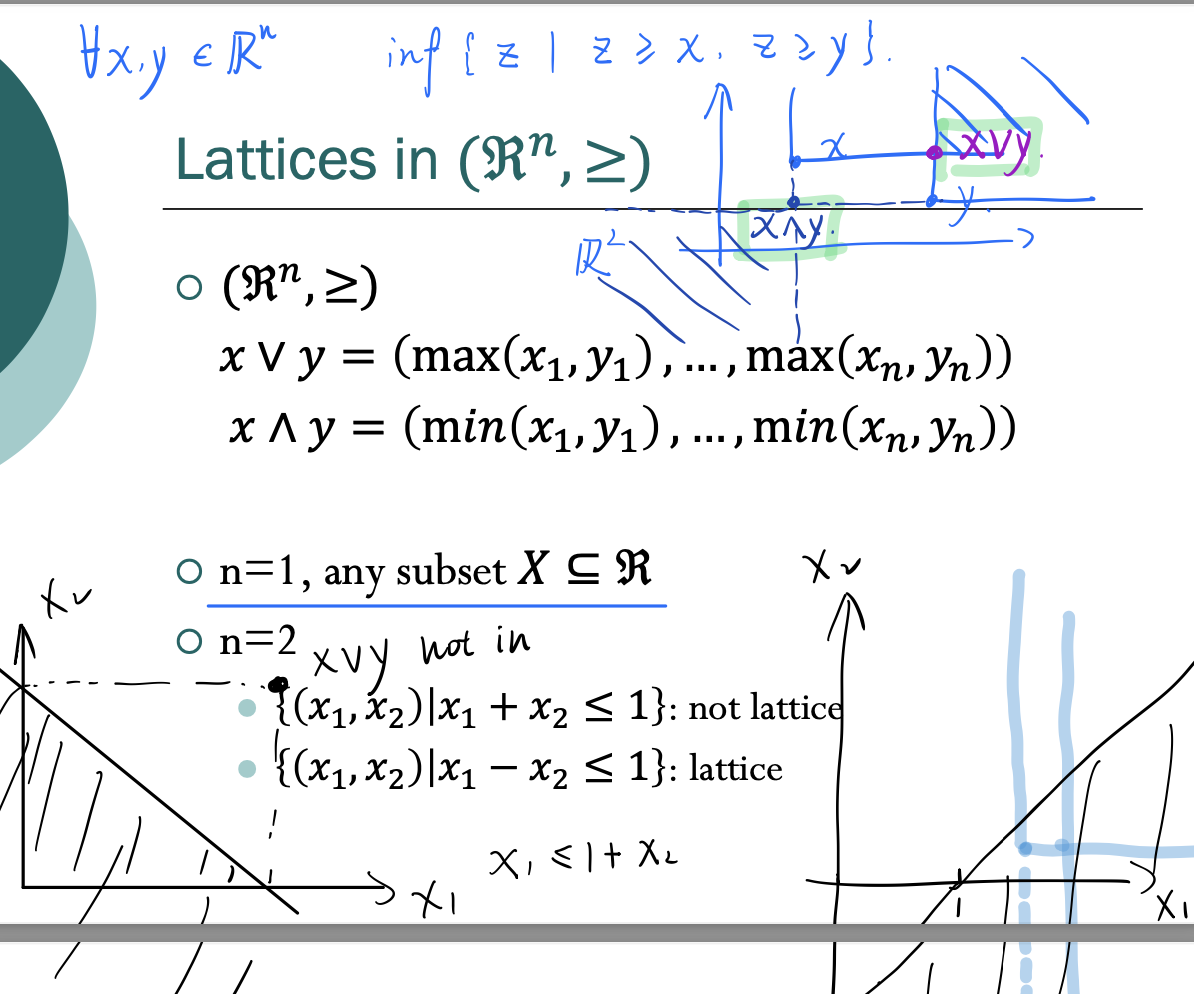
\includegraphics[scale=0.5]{lattice1.png}
    \caption{}
    \label{}
\end{figure}\end{center}

\begin{example}
Lattices:
\begin{enumerate}
    \item $\{0,1\}^n$
    \item $Z^n$
    \item a chain is a lattice (whose elements are ordered)
    \item Intersection of two lattices
\end{enumerate}
\end{example}

\subsection{Supermodularity}
\subsubsection{Definition: Supermodular $g(x \vee y)+g(x \wedge y) \geq g(x)+g(y), \forall x, y \in X$}
\begin{definition}
    A function $g: X \rightarrow \bar{\Re}(=\Re \cup\{+\infty\})$ is submodular if $$g(x \vee y)+g(x \wedge y) \leq g(x)+g(y), \forall x, y \in X$$
    $g$ is supermodular if $-g$ is submodular.
\end{definition}
\begin{center}
    \begin{tikzpicture}[domain=0:3.25]
    \draw[-](0,0)--(4,0) node[below] {$y$};
    \draw[-](4,0)--(4,2) node[above] {$x\vee y$};
    \draw[-](4,2)--(0,2) node[above] {$x$};
    \draw[-](0,2)--(0,0) node[below] {$x\wedge y$};
    \end{tikzpicture}
\end{center}
\begin{claim}
    $\operatorname{dom}(g)=\{x \in X \mid g(x)<+\infty\}$ is a lattice if $g$ is submodular.
\end{claim}
\begin{proof}
$\forall x,y\in \operatorname{dom}(g)$, prove $g(x\vee y)<+\infty$, $g(x\wedge y)<+\infty$.
\end{proof}

\subsubsection{Lemma: Supermodular $\Leftrightarrow$ $
\frac{\partial^{2} g(x)}{\partial x_{i} \partial x_{j}} \geq 0, \forall i \neq j
$}
\begin{lemma}
    Suppose $g$ is twice partially differentiable in $\mathfrak{R}^{n}$. Then $g$ is supermodular if and only if it has nonnegative cross partial derivatives, i.e.,
    $$
    \frac{\partial^{2} g(x)}{\partial x_{i} \partial x_{j}} \geq 0, \forall i \neq j
    $$
\end{lemma}
\begin{proof}
\quad

\begin{center}
        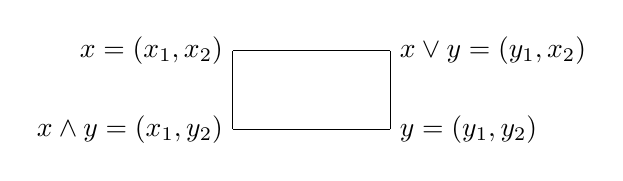
\begin{tikzpicture}[domain=0:3.25]
    \draw[-](0,0)--(2,0) node[right] {$y=(y_1,y_2)$};
    \draw[-](2,0)--(2,1) node[right] {$x\vee y=(y_1,x_2)$};
    \draw[-](2,1)--(0,1) node[left] {$x=(x_1,x_2)$};
    \draw[-](0,1)--(0,0) node[left] {$x\wedge y=(x_1,y_2)$};
    \end{tikzpicture}
\end{center}
$$x_1\leq y_1;\ y_2\leq x_2$$
\begin{equation}
    \begin{aligned}
        &g\text{ is supermodular}\\
        \Leftrightarrow	& g(x \vee y)-g(x)\geq g(y)-g(x \wedge y), \forall x, y \in X\\
        & g(y_1,x_2)-g(x_1,x_2)\geq g(y_1,y_2)-g(x_1,y_2), \forall x, y \in X\\
        &(\text{if }y_1 \rightarrow	x_1,\text{ $y_2$ kept unchanged})\\
        &\frac{\partial g(x_1,x_2)}{\partial x_1}\geq \frac{\partial g(x_1,y_2)}{\partial x_1}\\
        &(\text{if }y_2 \rightarrow	x_2,\ y_2\leq x_2)\\
        &\frac{\partial^2 g(x)}{\partial x_i\partial x_j}\geq 0,\ \forall i\neq j\\
    \end{aligned}
    \nonumber
\end{equation}
\end{proof}
\textbf{Note}: Supermodularity $\approx$ Economic Complementarity

$g$ is the profit function of selling products $x_1$ and $x_2$, $\frac{\partial}{\partial x_2}(\frac{\partial g(x_1,x_2)}{\partial x_1})\geq 0$

\begin{example}[Examples of Supermodular Functions]
    \quad

\begin{enumerate}
    \item $f(x)=x_{1}^{\alpha_{1}} x_{2}^{\alpha_{2}} \ldots x_{n}^{\alpha_{n}}\left(\alpha_{i} \geq 0\right)$ for $x \geq 0$
    \item $f(x, z)=\sum_{i=1}^{n} g_{i}\left(\alpha_{i} x_{i}-\beta_{i} z_{i}\right)$ for any univariate concave function $g_{i}: \Re \rightarrow \bar{\Re}\left(\alpha_{i} \beta_{i} \geq\right.$ $0)$
    \item $f(x)=\sum_{i, j=1}^{n} a_{i j} x_{i} x_{j}=x^TAx$ with $a_{i j}=a_{j i}$ is supermodular if and only if $a_{i j} \geq 0\ \forall i \neq j$
\end{enumerate}
\end{example}

\subsubsection{Lemma: Preservation of Supermodularity}
\begin{lemma}[Preservation of Supermodularity]
\quad

\begin{enumerate}[a)]
    \item If $f_{i}$ is supermodular, then $\lim _{i \rightarrow \infty} f_{i}(x), \sum_{i} \alpha_{i} f_{i}\left(\alpha_{i} \geq 0\right)$ are supermodular
    \item If $f: \Re \rightarrow \Re$ is convex and nondecreasing (nonincreasing) and $g: \Re^{n} \rightarrow \Re$ is increasing and supermodular (submodular), then $f(g(x))$ is supermodular
    \item Given $f: \Re^{n} \times \Re^{m} \rightarrow \Re$, if $f(\cdot, y)$ is supermodular for all $y$, then $E_{\xi}[f(x, \xi)]$ is supermodular in $x$
\end{enumerate}
\end{lemma}

\begin{lemma}[Supermodularity of composite functions]
    \quad

    If $X=\Pi_{i=1}^{n} X_{i}$ and $X_{i} \subseteq \Re, f_{i}\left(x_{i}\right): X_{i} \rightarrow \Re$ is increasing (decreasing) on $X_{i}$ for $i=1, \ldots, n$, and $g\left(z_{1}, \ldots, z_{n}\right): \Re^{n} \rightarrow \bar{\Re}$ is supermodular in $\left(z_{1}, \ldots, z_{n}\right)$, then
$$
g\left(f_{1}\left(x_{1}\right), \ldots, f_{n}\left(x_{n}\right)\right)
$$
is supermodular on $X$
\end{lemma}

\begin{lemma}[Topkis 1998]
    If $X$ is a lattice, $f_{i}(x)$ is increasing and supermodular (submodular) on $X$ for $i=$ $1, \ldots, k, Z_{i}$ is a convex subset of $R^{1}$ containing the range of $f_{i}(x)$ on $X$ or $i=1, \ldots, k$, and $g\left(z_{1}, \ldots, z_{k}, x\right)$ is supermodular in $\left(z_{1}, \ldots, z_{k}, x\right)$ and is increasing (decreasing) and convex in $z_{i}$ for fixed $z_{-i}$ and $x$, then $g\left(f_{1}(x), \ldots, f_{k}(x), x\right)$
is supermodular on $X$
\end{lemma}

\subsection{Parametric Optimization Problems}
\begin{definition}
    \begin{align*}
        f(s)=&\max g(s,a)\\
        &\text{s.t. }a\in A(s)
    \end{align*}
\end{definition}
$S$: subset of $\mathfrak{R}^{m}$
    
$A(s):$ finite dimensional

$C:=\{(s, a) \mid s \in S, a \in A(s)\}$ (the graph of the constraint operator)

$A^{*}(s)$, the optimal solution set, is nonempty for every $s \in S$

\begin{definition}
A set $A(s)$ is \textbf{ascending on $S$} if for $s\leq s'$, $a\in A(s)$, $a'\in A(s')$, we have $a\wedge a'\in A(s)$ and $a\vee a'\in A(s')$.
\end{definition}

\begin{example}
$A(s)=[s,+\infty)$ is ascending on $S$.
\end{example}




\subsubsection{Theorem: Maximizer of supermodular func is ascending, the maximum value is also supermodular}

\begin{theorem}[Ascending Optimal Solutions and Preservation]
    \quad

    If
    \begin{enumerate}
        \item $S$: sublattice of $\Re^{m}$
        \item $C:=\{(s, a) \mid s \in S, a \in A(s)\}$ is a sublattice
        \item $g$ is supermodular on $C$
    \end{enumerate}
    Then

    \begin{enumerate}
        \item $A^{*}(s)$ is \textbf{ascending} on $S$. Under some conditions, the largest/smallest element of $A^{*}(s)$ exists, and is increasing in $\mathrm{s}$.
        \item $f(s)$ is supermodular.
    \end{enumerate}
\end{theorem}

\begin{proof}
Take $s\leq s'$, $a^*\in A^*(s),\ {a'}^*\in A^*(s')$, i.e.
\begin{center}
    $g(s,a^*)=\max g(s,a)$ s.t. $a\in A(s)$\\
    $g(s',{a'}^*)=\max g(s',a)$ s.t. $a\in A(s')$
\end{center}
\begin{center}
    $(s,a^*)\vee(s',{a'}^*)=(s',a^*\vee{a'}^*)$\\
    $(s,a^*)\wedge(s',{a'}^*)=(s,a^*\wedge{a'}^*)$
\end{center}
As we know $C$ is a sublattice, we have
\begin{equation}
    \begin{aligned}
        (s',a^*\vee{a'}^*)\in C \Rightarrow	a^*\vee{a'}^*\in A(s')\\
        (s,a^*\wedge{a'}^*)\in C \Rightarrow	a^*\wedge{a'}^*\in A(s)
    \end{aligned}
    \nonumber
\end{equation}
Hence, $$g(s',a^*\vee{a'}^*)\leq g(s',{a'}^*);\ g(s,a^*\wedge{a'}^*)\leq g(s,a^*)$$
Since $g$ is supermodular on $C$,
\begin{equation}
    \begin{aligned}
        g(s',a^*\vee{a'}^*)+g(s,a^*\wedge{a'}^*)&\geq g(s,a^*)+g(s',{a'}^*)\\
        0\geq g(s',a^*\vee{a'}^*)-g(s',{a'}^*)&\geq g(s,a^*)-g(s,a^*\wedge{a'}^*)\leq 0
    \end{aligned}
    \nonumber
\end{equation}
Hence, $$g(s',a^*\vee{a'}^*)=g(s',{a'}^*);\ g(s,a^*)=g(s,a^*\wedge{a'}^*)$$
which means,
$$a^*\vee{a'}^*\in A^*(s'),\ a^*\wedge{a'}^*\in A^*(s)$$
Then, " $A^*(s)$ is ascending on $S$ " is proved.

What's more, the largest elements of $A(s')$ and $A(s)$ are $a^*\vee{a'}^*$ and $a^*$, the smallest elements of $A(s')$ and $A(s)$ are ${a'}^*$ and $a^*\wedge{a'}^*$, which are both increased as $s$ increases to $s'$.
\end{proof}

\begin{proof}
$\forall s,s'\in S$, $a\in A^*(s),a'\in A^*(s')$.
\begin{equation}
    \begin{aligned}
        f(s)+f(s')&=g(s,a)+g(s,a')\\
        &\text{(Since $g$ is supermodular on $C$)}\\
        &\leq g(s\wedge s',a\wedge a')+g(s\vee s',a\vee a')\\
        &\leq f(s\wedge s')+f(s\vee s')
    \end{aligned}
    \nonumber
\end{equation}
" $f(s)$ is supermodular " is proved.
\end{proof}

\begin{example}
    Pricing: 
$p^*(c)=\argmax_{p\geq c'}(p-c)D(p)$, $(c'>c)$
\end{example}
1. $C=\{(p,c)|c<c',p\geq c'\}$ is a sublattice of $\mathbb{R}^2$.

2. $g(p,c)=(p-c)D(p)$, $\frac{\partial^2 g(p,c)}{\partial p\partial c}=-D'(p)\geq 0$ $\Rightarrow$ $g$ is supermodular on $C$.

Hence, $p^*(c)$ is increasing in $c$.

\begin{example}
Newsvendor model: $\min_{x\geq 0}f(x)=cx+h_+E[(x-\xi)^+]+h_-E[(\xi-x)^+]$
\end{example}



\section{$L^\natural$-Convexity}
\subsection{Discrete Midpoint Convexity}
\begin{center}\begin{figure}[htbp]
    \centering
    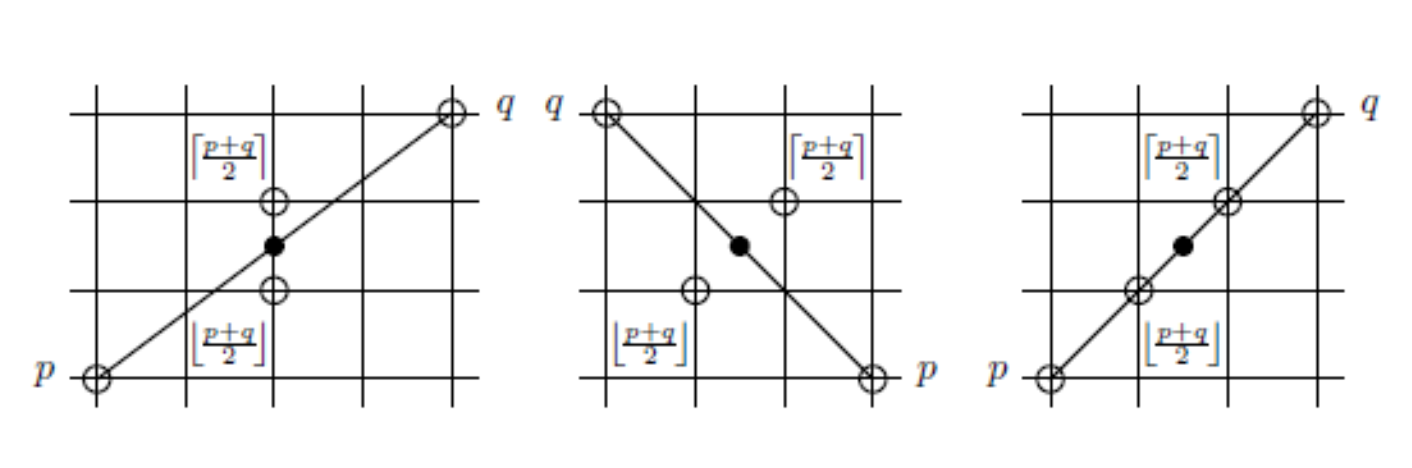
\includegraphics[scale=0.5]{DMC.png}
    \caption{Discrete Midpoint Convexity}
    \label{}
\end{figure}\end{center}
\begin{definition}
A function $f$ is \textbf{discrete midpoint convexity} if $$f(\lceil\frac{p+q}{2}\rceil)+f(\lfloor\frac{p+q}{2}\rfloor)\leq f(p)+f(q)$$
\end{definition}

\subsection{$L^\natural$-Convexity on $\mathbb{Z}^n$}
\begin{definition}
    A function $f: Z^{n} \rightarrow \bar{\Re}$ is called $L^{\natural}$ convex if $f$ satisfies the discrete midpoint convexity.
\end{definition}
\textbf{An equivalent definition}: A function $f: Z^{n} \rightarrow \bar{\Re}$ is $L^\natural$-convex if and only if
$$
g(x, \alpha):=f(x-\alpha e)=f([x_1-\alpha,x_2-\alpha,...,x_n-\alpha]^T)
$$
is submodular in $(x, \alpha)$ on $Z^{n+1}(e:$ all-ones vector $)$.





\subsection{$L^\natural$-Convexity on $\mathcal{F}^{n}(\mathcal{F}=\mathbb{Z}$ or $\Re)$}
\begin{definition}[Murota 2003]
    \quad

    A function $f: \mathcal{F}^{\mathrm{n}} \rightarrow \Re$ is \underline{$L^{\natural}$-convex if and only if $g(x, \xi):=f(x-\xi e)$ is submodular in $(x, \xi) \in \mathcal{F}^{\mathrm{n}} \times S$}, where $e$ is a vector with all components equal to 1 and $S$ is the intersection of $\mathcal{F}$ with any unbounded interval in $\mathfrak{R}$. $(f$ is required to be convex if $\mathcal{F}=\mathfrak{R})$
\end{definition}

\begin{definition}
    A set $V$ is \underline{$L^{\natural}$-convex if and only if its indicator function $\delta_V(x)$ is $L^{\natural}$.} $$\delta_V(x)=\left\{\begin{matrix}
        +\infty &,x\notin V\\
        0&, x\in V
    \end{matrix}\right.$$
    $\Leftrightarrow g(x,\xi)=\delta_V(x-\xi e)$ is subnormal, i.e.
    \begin{equation}
        \begin{aligned}
            g(x\vee y,\max\{\xi_x,\xi_y\})+g(x\wedge y,\min\{\xi_x,\xi_y\})\leq g(x,\xi_x)+g(y,\xi_y),\ \forall (x,\xi_x),(y,\xi_y)
        \end{aligned}
        \nonumber
    \end{equation}
    If $x-\xi_xe,y-\xi_y e$ in $V$, $x\vee y-\max\{\xi_x,\xi_y\}e\text{ and } x\wedge y-\min\{\xi_x,\xi_y\}$ must in $V$.
\end{definition}

Note: $f$ is $L^{\natural}$-concave if $-f$ is $L^{\natural}$-convex.


\subsection{Properties of $L^\natural$-Convexity}
\subsubsection{Proposition: $L^\natural$-convex $\Leftrightarrow$ $
a_{i j} \leq 0, \forall i \neq j, a_{i i} \geq 0, \sum_{j=1}^{n} a_{i j} \geq 0, \forall i
$}
\begin{proposition}
    A quadratic function $f(x)=\sum_{i, j=1}^{n} a_{i j} x_{i} x_{j}$ with $a_{i j}=a_{j i}$ is \underline{$L^\natural$-convex on $\mathcal{F}$ if and only if} its Hessian is a diagonally dominated M-matrix
    $$
    a_{i j} \leq 0\ \forall i \neq j,\quad a_{ii}\geq 0, \quad \sum_{j=1}^{n} a_{i j} \geq 0\ \forall i
    $$
\end{proposition}
\begin{proof}
\quad

$f(x)$ is $L^\natural$-convex $\Leftrightarrow$ $g(x,\xi)=f(x-\xi e)=\sum_{i,j=1}^na_{ij}(x_i-\xi)(x_j-\xi)$ is submodular in $(x,\xi)$ i.e.
\begin{equation}
    \begin{aligned}
        \frac{\partial^2 g}{\partial \xi\partial x_i}&=\frac{\partial}{\partial \xi}(\sum_{j=1}^na_{ij}(x_j-\xi)+\sum_{j=1}^na_{ji}(x_j-\xi))=-2\sum_{j=1}^na_{ij}\leq 0\\
        \frac{\partial^2 g}{\partial x_j\partial x_i}&=\frac{\partial}{\partial x_k}(\sum_{k=1}^na_{ik}(x_k-\xi)+\sum_{k=1}^na_{ki}(x_k-\xi))=2a_{ij}\leq 0
    \end{aligned}
    \nonumber
\end{equation}

\end{proof}



\begin{proposition}
    A twice continuous differentiable function $f: \Re^{n} \rightarrow \Re$ is \underline{$L^\natural$-convex if and only if} its Hessian is a diagonally dominated M-matrix, that is
    $$
    a_{i j} \leq 0, \forall i \neq j, a_{i i} \geq 0, \sum_{j=1}^{n} a_{i j} \geq 0, \forall i
    $$
\end{proposition}
\begin{proof}
\quad\\

$L^\natural$-convex $\Leftrightarrow$ $g(x,\xi)=f(x-\xi e)$ is subnormal

(if twice differentiable)

$\Leftrightarrow \frac{\partial^2 g(x,\xi)}{\partial x_i\partial x_j}=\frac{\partial^2 f(x-\xi e)}{\partial x_i\partial x_j}\leq 0, i\neq j$, $\frac{\partial^2 g(x,\xi)}{\partial x_i\partial \xi}=-\sum_{j=1}^n \frac{\partial^2 f(x-\xi e)}{\partial x_i\partial x_j}\leq 0$, $\forall (x,\xi)\in \Re^{n+1}$

$\Leftrightarrow \frac{\partial^2 f(x)}{\partial x_i\partial x_j}\leq 0, i\neq j;\ \sum_{j=1}^n \frac{\partial^2 f(x)}{\partial x_i\partial x_j}\geq 0$ $\forall x\in \Re^n$
\end{proof}

\subsubsection{Corollary: $L^{\natural}$-convex $\longrightarrow$ convex $+$ submodular}
\begin{corollary}
    If a twice differentiable function $f$ is $L^{\natural}$-convex, then the function is convex and submodular.
\end{corollary}
\begin{proof}
\quad\\
\underline{$a_{i j}=\frac{\partial^2 f(x)}{\partial x_i\partial x_j} \leq 0, i\neq j$} means the cross partial derivatives are nonpositive, which equals to \underline{$f$ is submodular}.
\begin{equation}
    \begin{aligned}
        x^T\nabla^2 f(x)x&=\sum_{i, j=1}^{n} a_{i j} x_{i} x_{j}\\
        &=\sum_k^na_{kk}x_k^2+\sum_{j=1}^n\sum_{i< j}a_{ij}2x_ix_j\\
        &\geq \sum_k^na_{kk}x_k^2+\sum_{j=1}^n\sum_{i< j}a_{ij}(x_i^2+x_j^2)\\
        &\geq \sum_k^{n-1}a_{kk}x_k^2+\sum_{j=1}^{n-1}\sum_{i< j}a_{ij}(x_i^2+x_j^2)\\
        &\cdots\\
        &\geq 0,\quad \forall x\in \Re^n
    \end{aligned}
    \nonumber
\end{equation}
Then $f$ is convex.
\end{proof}

\begin{example}
\end{example}
    - Given any univariate (discrete) convex function $g_{i}: \mathcal{F} \rightarrow \bar{\Re}$ and $h_{i j}: \mathcal{F} \rightarrow \Re$, the function $f: \mathcal{F}^{n} \rightarrow \bar{\Re}$ defined by
    $$
    f(x):=\sum_{i} g_{i}\left(x_{i}\right)+\sum_{i \neq j} h_{i j}\left(x_{i}-x_{j}\right)
    $$
    is $L^{\natural}$-convex.

\begin{example}
\end{example}
    - A set with a representation
    $$
    \left\{x \in \mathcal{F}^{n}: l \leq x \leq u, x_{i}-x_{j} \leq v_{i j}, i \neq j\right\}
    $$
    is $L^{\natural}$-convex, where $l, u \in \mathcal{F}^{n}, v_{i j} \in \mathcal{F}$.

\subsubsection{Theorem: Minimizer of $L^\natural$-convex func is nondecreasing with bounded sensitivity, the minimum value is also $L^\natural$-convex}
\begin{theorem}
Assume $g:\mathcal{F}^n\times \mathcal{F}^m \rightarrow	\overline{\Re}$ and set $C\subset \mathcal{F}^n\times \mathcal{F}^m$ are $L^\natural$-convex, define $$f(s)=\inf_{a:(s,a)\in C}g(s,a)$$
Then,
\begin{enumerate}
    \item The optimal solution set $A^*(s)$ is nondecreasing in $s$ with bounded sensitivity i.e., $$A^*(s+\omega e)\leq A^*(s)+\omega e,\ \forall \omega\in F_+$$ (Zipkin 2008, Chen et al. 2018)
    \item $f$ is $L^\natural-convex$. (Zipkin 2008)
\end{enumerate}
\end{theorem}

\subsection{Relationship with Multimodularity}
\begin{definition}
A function $f(x_1,x_2,...,x_n)$ is multimodular if $f(x_1-x_0,x_2-x_1,...,x_n-x_{n-1})$ submodular in $(x_0,x_1,...,x_n)$.
\end{definition}
Multimodularity and $L^\natural$-convexity are equivalent subject to an unimodular linear transformation.

\section{Optimization with decisions truncated by random variables}
$$\min_{u\in \mathcal{U}} E[f(u\wedge \xi)]$$
\textbf{Question 1 (Supply uncertainty in SCM):} $u$: ordering quantities; $\xi$: random capacities.

\textbf{Question 2 (Demand uncertainty in RM):} $u$: booking limits; $\xi$: random demands.

\textbf{Difficulty:} the object function is not convex (even if $f$ is).

\subsection{Unconstrained Problem}
Consider $$\tau^*=\min_{u\in \mathcal{F}^n} E[f(u\wedge \xi)]$$
$\mathcal{F}$ is either the real space or the set with all integers.

Random vector $\xi\in \mathcal{X}\subseteq \mathcal{F}^n$

\subsubsection{Reformulation}
\textbf{Reformulation:}
\begin{align*}
        &\min\quad E[f(v(\xi))]\\
        &\begin{array}{r@{\quad}r@{}l@{\quad}l}
        s.t.
        &v(\xi)&=(v_1(\xi_1),...,v_n(\xi_n))&, \forall \xi\in \mathcal{X} \\
        &v(\xi)&=u\wedge \xi&,\forall \xi\in \mathcal{X}\\
    \end{array} .
\end{align*}
Turn finding $u^*$ into finding $v^*()$

$v()$ is not convex.

\begin{theorem}[Equivalent Transformation, Chen, Gao and Pang 2018]
    Suppose that (Assumption I)

    (a) the function $f$ is lower semi-continuous with $f(u) \rightarrow+\infty$ for $|u| \rightarrow+\infty$;

    (b) the function $f$ is componentwise (discrete) convex;

    (c) the random vector $\xi$ has \underline{independent} components.

    Then $\tau^{*}$ is also the optimal objective value of the following optimization problem:
\begin{align*}
        &\min\quad E[f(v(\xi))]\\
        &\begin{array}{r@{\quad}r@{}l@{\quad}l}
        s.t.
        &v(\xi)&\leq \xi&,\forall \xi\in \mathcal{X}\\
        &v(\xi)&=(v_1(\xi_1),...,v_n(\xi_n))&, \forall \xi\in \mathcal{X} \\
    \end{array} .
\end{align*}
\end{theorem}

\subsubsection{$n=1$}
$\hat{u}$: minimizer of $f(u)$

Need to show $$\min_u E[f(u\wedge\xi)]=\min_{v(\xi)\leq \xi} E[f(v(\xi))]$$
\begin{center}\begin{figure}[htbp]
    \centering
    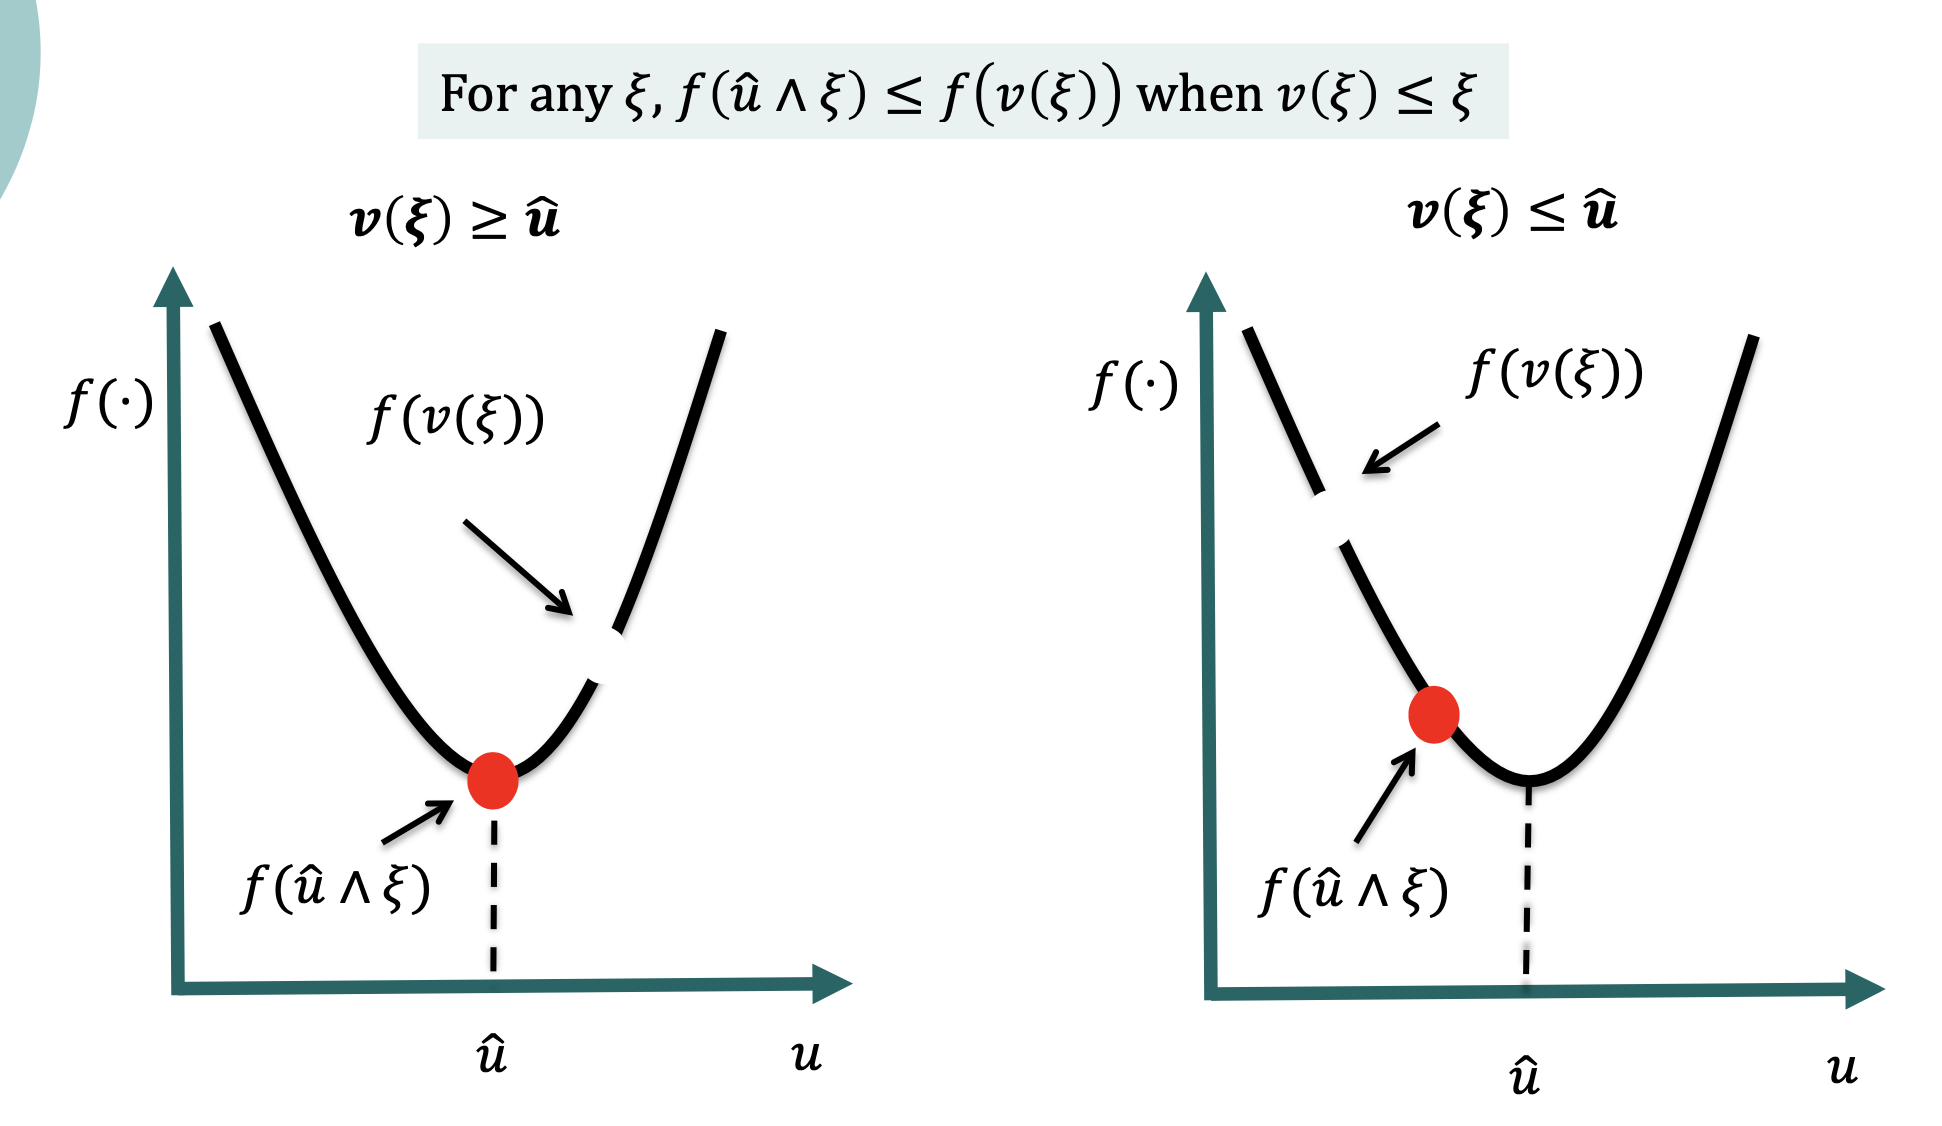
\includegraphics[scale=0.4]{leq.png}
    \caption{Easy to show $\forall \xi,\ f(\hat{u}\wedge\xi)\leq f(v(\xi))$ when $v(\xi)\leq \xi$}
    \label{}
\end{figure}\end{center}

Easy to show $\forall \xi,\ f(\hat{u}\wedge\xi)\leq f(v(\xi))$ when $v(\xi)\leq \xi$. Then $$\argmin E[f(u\wedge \xi)]=\hat{u}=\argmin f(u)$$
\begin{equation}
    \begin{aligned}
        E[f(\hat{u}\wedge\xi)]&\geq \min_uE[f(u\wedge\xi)]\\
        &\geq \min_{v(\xi)\leq \xi}E[f(v(\xi))]\text{ (Consider $v^*(\xi)\geq u$)}\\
        &\geq E[f(\hat{u}\wedge\xi)]\text{ (See the figure)}\\
        \Rightarrow	\quad &\min_u E[f(u\wedge\xi)]=\min_{v(\xi)\leq \xi} E[f(v(\xi))]
    \end{aligned}
    \nonumber
\end{equation}

\subsubsection{$n\geq 2$}
$$\argmin E[f(u\wedge \xi)]\neq \hat{u}$$
\begin{example}
$$f(u_1,u_2)=(u_1+u_2-2)^2+(u_1-1)^2+(u_2-1)^2$$
$\xi_1,\xi_2$ can take values $0$ and $2$ with equal probability.

$\hat{u}=(1,1)$

$\argmin E[f(u\wedge \xi)]=(1.2,1.2)$
\end{example}

\subsection{Transformation for Constrained Problem}
$$\min_{u\in \mathcal{U}} E[f(u\wedge \xi)]$$
$$\downarrow $$
\begin{align*}
    &\min\quad E[f(v(\xi))]\\
    &\begin{array}{r@{\quad}r@{}l@{\quad}l}
    s.t.
    &v(\xi)&\leq \xi&,\forall \xi\in \mathcal{X}\\
    &v(\xi)&=(v_1(\xi_1),...,v_n(\xi_n))\in \mathcal{V}&, \forall \xi\in \mathcal{X} \\
    &\mathcal{V}&=\{u\wedge\xi\ | u\in \mathcal{U},\xi\in \mathcal{X}\}&
\end{array} .
\end{align*}
\textbf{Sufficient Conditions for the Transformation}
\begin{enumerate}[(a)]
    \item $\mathcal{U}=\{u|Au\leq b,u\geq l\}$, where $A\geq 0$
    \item $\mathcal{X}_j\subseteq[l_j,+\infty)$
\end{enumerate}
(Example: some situations $l=(l_1,...,l_n)=(0,...,0)$)

\subsection{Generalization}
$$\min_{u\in \mathcal{F}^n} l(u)+E[f(u\wedge \xi)]$$
\begin{enumerate}[$\bullet$]
    \item $l:\mathcal{F}^n \rightarrow \bar{\Re}$, $f:\mathcal{F}^n \rightarrow \bar{\Re}$
    \item $\xi\in \mathcal{X}\subseteq \mathcal{F}^n$
    \item $\xi$ \textbf{dependent} (different from before !)
\end{enumerate}

\subsubsection{Positive Dependence}
Let $F_{\xi_{i}}$ be the joint CDF of $\xi_{1}, \ldots, \xi_{i-1}, \xi_{i+1}, \ldots, \xi_{n}$ conditioned on $\xi_{i}$

$\left\{\xi_{1}, \ldots, \xi_{i-1}, \xi_{i+1}, \ldots, \xi_{n} \mid \xi_{i}\right\}$ is \underline{stochastically increasing} if
$\int_{S} d F_{\xi_{i}}(w)$ is an increasing function of $\xi_{i}$ for each increasing set $S$

$\left\{\xi_{1}, \ldots, \xi_{i-1}, \xi_{i}, \xi_{i+1}, \ldots, \xi_{n}\right\}$ has \underline{positive dependence} if
$\left\{\xi_{1}, \ldots, \xi_{i-1}, \xi_{i+1}, \ldots, \xi_{n} \mid \xi_{i}\right\}$ is stochastically increasing for all $i$

\begin{proposition}
    The collection of random variables generated by nonnegative linear combination of \textbf{independent log-concave} random variables has positive dependence.
\end{proposition}

\subsubsection{Transformation}
\begin{theorem}[Equivalent Transformation, Chen and Gao 2018]
    Suppose that (Assumption II)
    \begin{enumerate}[(1)]
        \item the function $f$ is lower semi-continuous with $f(u) \rightarrow+\infty$ for $|u| \rightarrow+\infty$;
        \item the function $f$ is componentwise (discrete) convex and \underline{supermodular};
        \item the random vector $\xi$ is \underline{positive dependent};
        \item $l(u)$ is componentwise increasing.
    \end{enumerate}
    Then problem $\min _{u \in \mathcal{F}} l(u)+E[f(u \wedge \xi)]$ has the \textbf{same optimal objective value} of
    \begin{align*}
        &\min\quad l(u)+E[f(v(\xi))]\\
        &\begin{array}{r@{\quad}r@{}l@{\quad}l}
        s.t.
        &v(\xi)&\leq \xi&,\forall \xi\in \mathcal{X}\\
        &v(\xi)&\leq u&,\forall \xi\in \mathcal{X}\\
        &v(\xi)&=(v_1(\xi_1),...,v_n(\xi_n))&, \forall \xi\in \mathcal{X} \\
        &v_i(\xi_i)&\text{ is increasing for all }i&\\
    \end{array} .
\end{align*}
\end{theorem}

\section{Single-Leg Capacity Allocation}
(Seats reserved for future consumers)
\subsection{Two-Class Model}
Two periods: Period 1, random demand $D_2$ for price $p_2$; Period 2, random demand $D_1$ for price $p_1$. $p_1>p_2$

Provide $y$ in period 1 and the remaining will be provided in period 2.
\begin{align*}
    &\max\quad p_1E_{D_1,D_2}[D_1\wedge (c-(c-y)\wedge D_2)]+p_2E_{D_2}[(c-y)\wedge D_2]\\
    &\begin{array}{r@{\quad}r@{}l@{\quad}l}
    s.t.
    &0\leq y\leq c&,y\in \mathcal{F} &\\
\end{array} .
\end{align*}
Where $\mathcal{F}=\mathbb{R}$ or $\mathbb{Z}$ and $a\wedge b=\min(a,b)$

\subsubsection{Theorem: convex $f$, $\argmin E_{D}f(u\wedge D)=\argmin f(u)$}
When $D_2$ is sufficiently high. Let $b=c-y$, and the question transferred to
\begin{align*}
    &\max\quad v(b)=p_1E_{D_1}[D_1\wedge (c-b)]+p_2b\\
    &\begin{array}{r@{\quad}r@{}l@{\quad}l}
    s.t.
    &0\leq b\leq c&,b\in \mathcal{F} &\\
\end{array} .
\end{align*}
$v(b)$ is a concave function.

\begin{theorem}
Consider the following optimization problem
\begin{align*}
    &\min\quad E_{D}f(u\wedge D)\\
    &\begin{array}{r@{\quad}r@{}l@{\quad}l}
    s.t.
    &0\leq u\leq c&,u\in \mathcal{F} &\\
\end{array} .
\end{align*}
Assume $D$ is a nonnegative random variable.

If $f$ is \textbf{convex} and $\mathcal{F}=\mathbb{R}$ or $f$ is \textbf{discrete convex} and $\mathcal{F}=\mathbb{Z}$, then any optimal solution of
\begin{align*}
    &\min\quad f(u)\\
    &\begin{array}{r@{\quad}r@{}l@{\quad}l}
    s.t.
    &0\leq u\leq c&,u\in \mathcal{F} &\\
\end{array} .
\end{align*}
is also optimal for the former optimization problem.

\textbf{(Actually, quasi-convexity suffices)}
\end{theorem}
According to the $n=1$ discussion of section 3, the theorem is easy to be proved. Then, the global-max in $v(b)$ is global-max for objective function.

Then we consider the equivalent minimum problem,
\begin{align*}
    &\max\quad \phi(y)=p_2y-p_1E_{D_1}[D_1\wedge y]\\
    &\begin{array}{r@{\quad}r@{}l@{\quad}l}
    s.t.
    &0\leq y\leq c&,y\in \mathcal{F} &\\
\end{array} .
\end{align*}
We need to find the optimal $y^*$ minimize the $\phi(y)$. To simplify the analysis, we find the $y^\circ$ which is the optimal $y$ regardless constraints. $y^*=\left\{\begin{matrix}
    0& \text{ if }y^\circ<0\\
    y^\circ&\text{ if }y^\circ\in[0,c]\\
    c&\text{ if }y^\circ>c
\end{matrix}\right.$
\subsubsection{Discrete, $\mathcal{F}=\mathbb{Z}$}
\begin{equation}
    \begin{aligned}
        \phi(y)-\phi(y-1)=p_2-p_1P(D_1\geq y)
    \end{aligned}
    \nonumber
\end{equation}
Then, the $y^\circ$ is
\begin{equation}
    \begin{aligned}
        \overline{y}&=\min\{y\in \mathbb{Z}: P(D_1>y)<r\}\\
        \underline{y}&=\max\{y\in \mathbb{Z}: P(D_1\geq y)>r\} \textbf{ (Littlewood's rule)}\\
        y^\circ&=[\underline{y},\overline{y}]\cap \mathbb{Z}
    \end{aligned}
    \nonumber
\end{equation}
Where $r=\frac{p_2}{p_1}$, higher $r$ causes lower $y^\circ$.

\begin{example}
    Suppose that $D_1$ is a Poisson random variable with mean 80, the full fare is $p_1 = 100$ and the discounted fare is $p_2 = 60$
\end{example}
$r=60/100=0.6$, $y^*=\max\{y\in \mathbb{Z}: P(D_1\geq y)>r\}=78$







\subsubsection{Continuous, $\mathcal{F}=\mathbb{R}$}
$y^\circ$ is the $y$ s.t. $1-F_1(y)=r$, where $F_1(\cdot)$ is the CDF of $D_1$.
$$y^\circ=F_1^{-1}(1-r)$$
\textbf{Special Case:} $D_1\sim \mathcal{N}(\mu,\sigma^2)$
\begin{equation}
    \begin{aligned}
        F_1(y)=\varPhi(\frac{y-\mu}{\sigma})
    \end{aligned}
    \nonumber
\end{equation}
$\varPhi(\cdot)$ is the CDF of the standard normal $\mathcal{N}(0,1)$. Then,
\begin{equation}
    \begin{aligned}
        y^\circ=\mu+\sigma\varPhi^{-1}(1-r)
    \end{aligned}
    \nonumber
\end{equation}
If $\frac{p_2}{p_1}=r<\frac{1}{2}$, $y^\circ$ increases as variance $\sigma$ increases.

\subsection{Multi-Class Model}
\begin{enumerate}[$\bullet$]
    \item $p_1>p_2>\cdots>p_n$
    \item Lower class demand arrives earlier.
    \item Demand of different classes are independent.
    \item Control: demand to accept or reject.
\end{enumerate}
\subsubsection{Sequence of Events}
At stage $j$ with remaining capacity $x$,
\begin{enumerate}
    \item Select booking limit $b$ for class $j$, equivalently, protection level $y=x-b$ for classes $l$, $l<j$.
    \item Demand $D_j$ is realized.
    \item Accept $b\wedge D_j$ of class $j$ and collect revenue $p_j(b\wedge D_j)$.
    \item Move on to stage $j-1$ with remaining capability $x-b\wedge D_j$.
\end{enumerate}

\subsubsection{Dynamic Programming}
Set $f_j(x,b)=p_j b+V_{j-1}(x-b)$, $V_0(x)=0, V_j(0)=0$, $x=0,1,...,c\text{ (discrete)}$, $x\in[0,c]\text{ (continuous)}$
\begin{equation}
    \begin{aligned}
        V_j(x)=\max_{b\in[0,x],b\in \mathcal{F}} \mathbb{E}[f_j(x,b\wedge D_j)]
        =\mathbb{E}[p_j (b\wedge D_j)]+\mathbb{E}[V_{j-1}(x-b\wedge D_j)]
    \end{aligned}
    \nonumber
\end{equation}
\begin{proposition}
(1). $\forall j$, $f_j$ is $L^\natural-$concave, $V_j$ is (discrete) convex; (2). The optimal solution of the dynamic programming $b_j^*$ is the same as $$\max_{b\in[0,x],b\in \mathcal{F}} f_j(x,b)=p_j b+V_{j-1}(x-b)$$
\end{proposition}
Define $y^*_{j-1}$ be the optimal solution of
$$\max_{y\geq 0,y\in \mathcal{F}} -p_j y+V_{j-1}(y)$$
Then $$b_j^*=(x-y_{j-1}^*)^+$$

\begin{equation}
    \begin{aligned}
        V_j(x)&=\mathbb{E}[f_j(x,(x-y_{j-1}^*)^+\wedge D_j)]\\
        &=\mathbb{E}[p_j(x-y_{j-1}^*)^+\wedge D_j+V_{j-1}(x-(x-y_{j-1}^*)^+\wedge D_j)]\\
        &=\left\{\begin{matrix}
            V_{j-1}(x)&\text{ if }x\leq y_{j-1}^*\\
            \mathbb{E}[p_j(x-y_{j-1}^*)\wedge D_j+V_{j-1}(x-(x-y_{j-1}^*)\wedge D_j)]&\text{ if }x> y_{j-1}^*
        \end{matrix}\right.
    \end{aligned}
    \nonumber
\end{equation}

\subsection{Discrete Case}
Define
\begin{equation}
    \begin{aligned}
        \Delta V_j(x)&=V_j(x)-V_j(x-1)
    \end{aligned}
    \nonumber
\end{equation}



\begin{lemma}
    If $x> y^*_{j-1}$, $\Delta V_j(x)=\mathbb{E}[\min\{p_j,\Delta V_{j-1}(x-D_j)\}]$
\end{lemma}
\begin{proof}
\quad\\
\begin{equation}
    \begin{aligned}
        \Delta V_j(x)&=p_j(\mathbb{E}[(x-y_{j-1}^*)\wedge D_j]-\mathbb{E}[(x-1-y_{j-1}^*)\wedge D_j])\\&+\mathbb{E}[V_{j-1}(x-(x-y_{j-1}^*)\wedge D_j)]-\mathbb{E}[V_{j-1}(x-1-(x-1-y_{j-1}^*)\wedge D_j)]\\
        &=\left\{\begin{matrix}
        p_j    &\text{ if }x-y^*_{j-1}\leq D_j\\
        \Delta V_{j-1}(x-D_j)    &\text{ if }x-y^*_{j-1}> D_j
        \end{matrix}\right.\\
        &=\mathbb{E}[p_j \mathbb{I}(x-D_j\leq y_{j-1}^*)+\Delta V_{j-1}(x-D_j)\mathbb{I}(x-D_j> y_{j-1}^*)]\\
        &(\text{ Since $y_{j-1}^*$ maximizes $-p_j y+V_{j-1}(y)$,}\\&\text{ $\Delta V_{j-1}(y)> p_j$ if $y\leq y_{j-1}^*$ and $\Delta V_{j-1}(y)\leq p_j$ if $y> y_{j-1}^*$})\\
        &=\mathbb{E}[\min\{p_j,\Delta V_{j-1}(x-D_j)\}]\\
    \end{aligned}
    \nonumber
\end{equation}
\end{proof}



\begin{proposition}[1.5 of GT 19]
    \quad

    \begin{enumerate}[(i)]
        \item $\Delta V_j(x+1)\leq \Delta V_j(x)$ (proved by $V_j$ is discrete concave)
        \item $\Delta V_{j+1}(x)\geq \Delta V_{j}(x)$
    \end{enumerate}
\end{proposition}
\begin{proof}
\quad\\
If $x\leq y^*_{j-1}$,
\begin{equation}
    \begin{aligned}
        \Delta V_j(x)&=V_{j-1}(x)-V_{j-1}(x-1)=\Delta V_{j-1}(x)
    \end{aligned}
    \nonumber
\end{equation}
If $x> y^*_{j-1}$ (i.e. $x-1\geq y^*_{j-1}$),
\begin{equation}
    \begin{aligned}
        \Delta V_j(x)
        &=\mathbb{E}[\min\{p_j,\Delta V_{j-1}(x-D_j)\}]\\
        &(\text{ $V_{j-1}(x)$ is discrete concave})\\
        &\geq \mathbb{E}[\min\{p_j,\Delta V_{j-1}(x)\}]\\
        &(\text{ Since $x>y_{j-1}^*$, $V_{j-1}(x)< p_j$})\\
        &=\Delta V_{j-1}(x)
    \end{aligned}
    \nonumber
\end{equation}
\end{proof}

\begin{theorem}[part of 1.6 of GT 19]
    \quad

    The optimal protection level at stage $j$ is $$y_{i-1}^*=\max\{y\in \mathbb{N}_+: \Delta V_{j-1}(y)>p_j \}$$
    Moreover, $y_{n-1}^*\geq y_{n-2}^*\geq \cdots \geq y_1^*=y_0^*=0$
\end{theorem}
(Easy to prove: Since $y_{j-1}^*$ maximizes $-p_j y+V_{j-1}(y)$, $\Delta V_{j-1}(y)> p_j$ if $y\leq y_{j-1}^*$ and $\Delta V_{j-1}(y)\leq p_j$ if $y> y_{j-1}^*$)

\textbf{Note:} Littlewood's rule is a special case for $n=2$.

\subsubsection{Discrete Case: Reformulation}
\begin{equation}
    \begin{aligned}
        V_j(x)&=\mathbb{E}[p_j(x-y_{j-1}^*)^+\wedge D_j+V_{j-1}(x-(x-y_{j-1}^*)^+\wedge D_j)]\\
        &=V_{j-1}(x)+\mathbb{E}[p_j(x-y_{j-1}^*)^+\wedge D_j+(V_{j-1}(x-(x-y_{j-1}^*)^+\wedge D_j)-V_{j-1}(x))]\\
        &=V_{j-1}(x)+\mathbb{E}[p_j(x-y_{j-1}^*)^+\wedge D_j-\sum_{z=1}^{(x-y_{j-1}^*)^+\wedge D_j}\Delta V_{j-1}(x+1-z)]\\
        &=V_{j-1}(x)+\mathbb{E}[\sum_{z=1}^{(x-y_{j-1}^*)^+\wedge D_j}(p_j-\Delta V_{j-1}(x+1-z))]\\
        V_j(x)&=V_{j-1}(x)+\mathbb{E}[\sum_{z=1}^{u^*}(p_j-\Delta V_{j-1}(x+1-z))]\\
        &u^*=\min\{(x-y_{j-1}^*)^+,D_j\}\\
        &y_{i-1}^*=\max\{y\in \mathbb{N}_+: p_j<\Delta V_{j-1}(y) \}
    \end{aligned}
    \nonumber
\end{equation}
\begin{enumerate}[$\bullet$]
    \item $y_1^*\leq y_2^*\leq \cdots\leq y_n^*$
    \item The "nested" booking limit $b_j^*=C-y_{j-1}^*$, $j=2,...,n$
    
    (nested booking limit is the total amount can be booked in $j,j+1,...,n$)
    $$b_j^*=y_j$$
    \item The marginal utility at $j$ of choosing to reserve one more item in the next stage $j-1$: $$\pi_j(x)=\Delta V_{j-1}(x)$$
    \item The amount of selling at stage $j$ $$u^*=\left\{\begin{matrix}
        0&\text{ if }p_j<\pi_j(x)\\
        \min\{\max\{z:p_j\geq \pi_j(x-z)\},D_j\}&\text{ if }p_j\geq \pi_j(x)
    \end{matrix}\right.$$
     $p_j<\pi_j(x)$ means the marginal utility of reserving is larger than selling it now.
\end{enumerate}

We can further compute, if $x>y_{j-1}^*$,
\begin{equation}
    \begin{aligned}
        \Delta V_j(x)=
            p_jPr(D_j\geq x-y_{j-1}^*)+\sum_{k=0}^{x-y_{j-1}^*-1}\Delta V_{j-1}(x-k)Pr(D_j=k)
    \end{aligned}
    \nonumber
\end{equation}
If $x\leq y_{j-1}^*$, $\Delta V_j(x)=\Delta V_{j-1}(x)$.

Which will simplify the computation.



\subsubsection{Discrete Case: Computation}

The policy is implemented as follows:
\begin{enumerate}
    \item At stage $n$, we start with $x_{n}=c$ units of inventory and we protect $y_{n-1}\left(x_{n}\right)=\min \left\{y_{n-1}^{*}, x_{n}\right\}$ units of capacity for fares $n-1, n-2, \ldots, 1$.
    \item Therefore, we allow up to $\left[x_{n}-y_{n-1}^{*}\right]^{+}$units of capacity to be sold to fare class $n$.
    \item We sell $\min \left\{\left[x_{n}-y_{n-1}^{*}\right]^{+}, D_{n}\right\}$ units of capacity to fare class $n$ and we have a remaining capacity of $x_{n-1}=x_{n}-\min \left\{\left[x_{n}-y_{n-1}^{*}\right]^{+}, D_{n}\right\}$ at stage $n-1$.
    \item We protect $y_{n-2}\left(x_{n-1}\right)=\min \left\{y_{n-2}^{*}, x_{n-1}\right\}$ units of capacity for fares $n-2, n-1, \ldots, 1$.
    \item Therefore, we allow up to $\left[x_{n-1}-y_{n-2}^{*}\right]^{+}$units of capacity to be sold to fare class $n-1$.
    \item We continue until we reach stage 1 with $x_{1}$ units of capacity, allowing $\left(x_{1}-y_{0}\right)^{+}=\left(x_{1}-0\right)^{+}=x_{1}$ to be sold to fare class $1$.
\end{enumerate}

\begin{equation}
    \begin{aligned}
        V_j(x)=\mathbb{E}[p_j\min\{(x-y_{j-1}^*)^+, D_j\}+V_{j-1}(x-\min\{(x-y_{j-1}^*)^+, D_j\})]
    \end{aligned}
    \nonumber
\end{equation}
$y_0^*=0, V_0(x)=0$, then we can compute $y_1^*,V_1(x)$,...

\textbf{Backward:}
Use
\begin{equation}
    \begin{aligned}
        \Delta V_j(x)&=
            p_jPr(D_j\geq x-y_{j-1}^*)+\sum_{k=0}^{x-y_{j-1}^*-1}\Delta V_{j-1}(x-k)Pr(D_j=k)\\
        y_{j-1}^*&=\max\{y\in \mathbb{N}_+: p_j<\Delta V_{j-1}(y) \}
    \end{aligned}
    \nonumber
\end{equation}
\begin{enumerate}
    \item $V_1(x_1)=\mathbb{E}[p_1\min\{x_1, D_1\}]$, then $\Delta V_{1}(x)=p_1 Pr(D_1\geq x)$
    \item $y_1^*=\max\{y\in \mathbb{N}_+: p_2<\Delta V_{1}(y) \}=\max\{y:Pr(D_1\geq y)>\frac{p_2}{p_1}\}$
    \begin{equation}
        \begin{aligned}
            \Delta V_2(x)&=p_2Pr(D_2\geq x-y_{1}^*)+\sum_{k=0}^{x-y_{1}^*-1}p_1 Pr(D_1\geq x-k)Pr(D_2=k)
        \end{aligned}
        \nonumber
    \end{equation}
    \item $y_2^*=\max\{y\in \mathbb{N}_+: p_3<\Delta V_{2}(y)\}=\max\{y: Pr(\Delta V_{1}(y-D_2)>p_3)\}$
    \item $\dots$
\end{enumerate}

The complexity is $O(nC^2)$

\begin{example}
    Suppose that there are five fare classes. The demand for all fare classes is a Poisson random variable. The fares and the expected demand for the
    five fare classes are given by $(p_5, p_4, p_3, p_2, p_1) = (15, 35, 40, 60, 100)$ and $(\mathbb{E}{D_5}, \mathbb{E}{D_4}, \mathbb{E}{D_3}, \mathbb{E}{D_2}, \mathbb{E}{D_1}) = (120, 55, 50, 40, 15)$. For this problem instance, the optimal protection levels are
\end{example}
\begin{enumerate}
    \item $V_1(x_1)=\mathbb{E}[100\min\{x_1, D_1\}]$, then $\Delta V_{1}(x)=100 Pr(D_1\geq x)$
    \item $y_1^*=\max\{y:Pr(D_1\geq y)>\frac{3}{5}\}=14$
    \begin{equation}
        \begin{aligned}
            \Delta V_2(x)&=60Pr(D_2\geq x-14)+\sum_{k=0}^{x-15}100 Pr(D_1\geq x-k)Pr(D_2=k)
        \end{aligned}
        \nonumber
    \end{equation}
    \item $y_2^*=\max\{y\in \mathbb{N}_+: p_j<$
\end{enumerate}



\subsection{Continuous Case}
Skip

\subsection{ Generalized Newsvendor Problem: High-before-low arrival pattern}
Consider the problem of selecting $c$ to maximize $$\Pi_n(c)=V_n(c)-kc$$
Where $V_n(c)$ is the expected revenue to the multi-fare RM problem.

Assume high-before-low arrival pattern. Then
$$V_n(c)=\sum_{j=1}^n p_j \mathbb{E}[D_j\wedge (c-D_{1:j-1})^+]$$
and $$\Delta V_n(c)=\sum_{j=1}^n(p_j-p_{j+1})Pr(D_{1:j}>c)$$
Where $D_{1:j}=\sum_{l=1}^j D_l, p_{n+1}=0$

\subsection{Heuristics}
When there are two classes, we find $y^*$: $\max\{y\in \mathbb{Z}: P(D_1\geq y)>r\}$

We try to use this form to simplify our computation,

\textbf{EMSR (expected marginal seat revenue)}
\begin{enumerate}[$\bullet$]
    \item \textbf{EMSR - a}
    \begin{equation}
        \begin{aligned}
            y_k^{j+1}&=\max\{y:P(D_k\geq y)>\frac{p_{j+1}}{p_k}\}, k=j,j-1,...,1\\
            y_j&=\sum_{k=1}^jy_k^{j+1}
        \end{aligned}
        \nonumber
    \end{equation}
    \item \textbf{EMSR - b}
    \begin{equation}
        \begin{aligned}
            \overline{p}_j&=\frac{\sum_{k=1}^jp_k \mathbb{E} [D_k]}{\sum_{k=1}^j \mathbb{E} [D_k]}\\
            y_j&=\max\{y:P(\sum_{k=1}^j D_k\geq y)>\frac{p_{j+1}}{\overline{p}_j}\}
        \end{aligned}
        \nonumber
    \end{equation}
\end{enumerate}

\subsection{ Bounds on Optimal Expected Revenue}
\subsubsection{Upper Bound}
\begin{equation}
    \begin{aligned}
        \overline{V}(c|D):&=\max\{\sum_{j=1}^np_jx_j|\sum_{j=1}^nx_j\leq c,0\leq x_j\leq D_j,j=1,...,n\}\\
        V_n^U(c):&=\mathbb{E}[\overline{V}(c|D)]\\
        &=\sum_{j=1}^n(p_j-p_{j+1})\sum_{k=1}^cPr(D_{1:j}\geq k),\quad (\text{Set }p_{n+1}=0)\\
        \mathbb{E}[\overline{V}(c|D)]&\leq \overline{V}(c|D)=\sum_{j=1}^n(p_j-p_{j+1})\min\{\overline{D}_{1:j},c\}
    \end{aligned}
    \nonumber
\end{equation}
\subsubsection{Lower Bound}
Using zero protection level
\begin{equation}
    \begin{aligned}
        V_n^L(c)&=\sum_{j=1}^n p_j \mathbb{E}[\min\{D_k,(c-D_{j+1:n})^+\}]\\
        &=\sum_{j=1}^n(p_j-p_{j-1})\mathbb{E}[\min\{D_{j:n},c\}],\quad (\text{Set }p_{0}=0)
    \end{aligned}
    \nonumber
\end{equation}


\subsection{Dynamical Models}
\begin{enumerate}[$\bullet$]
    \item $p_1\geq p_2\geq \cdots \geq p_n$.
    \item $T$ periods.
    \item At most one arrival each period.
    \item $\lambda_{jt}$: probability of an arrival of class $j$ in period $t$.
    \item $M_t$: set of offered classes.
\end{enumerate}

\subsubsection{Discrete Time}
\begin{equation}
    \begin{aligned}
        V_t(x)&=\sum_{j\in M_t}\lambda_{jt}\max\{p_j+V_{t-1}(x-1),V_{t-1}(x)\}+(1-\sum_{j\in M_t}\lambda_{jt})V_{t-1}(x)\\
        &=V_{t-1}(x)+\sum_{j\in M_t}\lambda_{jt}[p_j-\Delta V_{t-1}(x)]^+\\
        &=V_{t-1}(x)+R_t(\Delta V_{t-1}(x))
    \end{aligned}
    \nonumber
\end{equation}
Where we set $R_t(z)=\sum_{j\in M_t}\lambda_{jt}[p_j-z]^+$, $V_t(0)=0$, $V_0(x)=0,\forall x\geq 0$

\subsubsection{Continuous Time: Poisson arrival}
$$\frac{\partial V_t(x)}{\partial t}=R_t(\Delta V_t(x))$$

\subsubsection{Optimal Policy: discrete time}
Let $$a(t,x)=\max\{j:p_j\geq \Delta V(t-1,x)\}$$
Optimal to accept all fares in the active set
$$A(t,x)=\{j\in M_t: j\leq a(t,x)\}$$
and reject the remaining fare classes

\subsubsection{Structural Properties}
\begin{theorem}[1.18 of GT]
\quad

\begin{enumerate}[$\bullet$]
    \item $V_t(x)$ is increasing in $t,x$.
    \item $\Delta V_t(x)$ is increasing in $t$ and decreasing in $x$.
    \item $a(t,x),A(t,x)$ is increasing in $x$.
\end{enumerate}
If $\lambda_{jt}\equiv \lambda_j>0$, $M_t\equiv M=\{1,...,n\}$, then
\begin{enumerate}[$\bullet$]
    \item $V_t(x)$ is strictly increasing and concave in $t$.
    \item $a(t,x),A(t,x)$ is decreasing in $t$.
\end{enumerate}
\end{theorem}

\subsubsection{Discrete Case: Computation}
\begin{equation}
    \begin{aligned}
        V_t(x)=V_{t-1}(x)+\sum_{j\in M_t}\lambda_{jt}[p_j-\Delta V_{t-1}(x)]^+
    \end{aligned}
    \nonumber
\end{equation}
$V_0(x)=0$, then $V_1(x)$, then $\Delta V_1(x)$.

The complexity is $O(nC T)$ ($T \approx O(C)$)


\section{Network Revenue Management with Independent Demands}
\subsection{Settings}
\begin{enumerate}[$\bullet$]
    \item $m$ resources with initial capacities $c=\begin{pmatrix}
        c_1\\
        c_2\\
        \vdots\\
        c_m
    \end{pmatrix}\in \mathbb{Z}_+^m$
    \item Time from $T,T-1,T-2,...$ to $0$.
    \item ODF $kj$: Itineraries $k=1,...,K$; Possible fares for itinerary $k$, $p_{kj}$, $j\in \{1,...,n_k\}$. (Every itinerary may have $n_k$ kinds of prices).
    \item Demand arrives as compound Poisson arrival process with rate $\lambda_{tkj}$ at time $t$ for ODF $kj$.
    \item Resources utilized by itinerary $k$: $A_k=\begin{pmatrix}
        a_{1k}\\
        \vdots\\
        a_{mk}
    \end{pmatrix}$, $a_{ik}\in\{0,1\}$ with $a_{ik}=1$ if resource $i$ is consumed by itinerary $k$.
    \item $V(t,x)$: the maximum total expected revenue that can be extracted when the remaining capacities are $x\in \mathbb{Z}_+^m$ and the remaining time is $t\in \mathbb{R}_+$.
    \item Decision: $u=\{u_{kj}: j=1,...,n_k,k=1,...,K\}$, $u_{kj}=\left\{\begin{matrix}
        1& \text{accept a request for ODF }k_j\\
        0& \text{others}
    \end{matrix}\right.$
    \item Feasible set of decisions: $u(x)=\{u_{kj}\in\{0,1\}: A_ku_{kj}\leq x, j=1,...,n_k,k=1,...,K\}$
\end{enumerate}


\subsection{HJB Equation}
Assume now that the state is $(t, x)$ and consider a time increment $\delta t$ that is small enough so that we can approximate the probability of an arrival of a request for fare $j$ of itinerary $k$ by $\lambda_{tkj}\delta k$.

$$
\begin{aligned}
V(t, x)=& \sum_{k=1}^{K} \sum_{j=1}^{n_{k}} \lambda_{t k j} \delta t \max _{u_{k j} \in\{0,1\}}\left[p_{k j} u_{k j}+V\left(t-\delta t, x-A_{k} u_{k j}\right)\right] \\
&+\left\{1-\sum_{k=1}^{K} \sum_{j=1}^{n_{k}} \lambda_{t k j} \delta t\right\} V(t-\delta t, x)+o(\delta t)
\end{aligned}
$$
where $o(\delta t)$ is a quantity that goes to zero faster than $\delta t$. Subtracting $V(t-\delta t, x)$ from both side of the equation, dividing by $\delta t$, and using the notation $\Delta_{k} V(t, x)=$ $V(t, x)-V\left(t, x-A_{k}\right)$, we obtain the \underline{Hamilton-Jacobi-Bellman (HJB) equation}
$$
\frac{\partial V(t, x)}{\partial t}=\sum_{k=1}^{K} \sum_{j=1}^{n_{k}} \lambda_{t k j}\left[p_{k j}-\Delta_{k} V(t, x)\right]^{+}
$$
with boundary conditions $V(t, 0)=V(0, x)=0$ for all $t \geq 0$ and all $x \geq 0$. Notice that term $\left[p_{k j}-\Delta V_{k}(t, x)\right]^{+}$is equivalent to the maximum of $p_{k j} u_{k j}+V(t, x-$ $\left.A_{k} u_{k j}\right)-V(t-\delta t, x)$ over $u_{k j} \in\{0,1\} .$

For any vector $z \geq 0$, Define
$$
R_{t}(u, z):=\sum_{k=1}^{K} \sum_{j=1}^{n_{k}} \lambda_{t k j}\left[p_{k j}-z_{k}\right] u_{k j}
$$
and
$$
\begin{aligned}
\mathcal{R}_{t}(z):=\max _{u} R_{t}(u, z)=\sum_{k=1}^{K} \sum_{j=1}^{n_{k}} \lambda_{t k j} \max _{u_{j k} \in\{0,1\}}\left[p_{k j}-z_{k}\right] u_{k j}=\sum_{k=1}^{K} \sum_{j=1}^{n_{k}} \lambda_{t k j}\left[p_{k j}-z_{k}\right]^{+}
\end{aligned}
$$
Then $$
\frac{\partial V(t, x)}{\partial t}=\mathcal{R}_{t}(\Delta V(t, x)),\quad \Delta V(t, x)=\begin{pmatrix}
    \Delta_{1} V(t, x)\\
    \Delta_{2} V(t, x)\\
    \vdots\\
    \Delta_{K} V(t, x)\\
\end{pmatrix}
$$

\begin{center}
    \fcolorbox{black}{gray!10}{\parbox{.9\linewidth}{\begin{enumerate}
        \item Let's aggregate ODF's into a single index.
        \item $n=\sum_{k=1}^K n_k$
        \item HJB equation:
        $$\frac{\partial V(t, x)}{\partial t}=\mathcal{R}_{t}(\Delta V(t, x))=\sum_{j\in M_t} \lambda_{t j}\left[p_{j}-\Delta_jV(t,x)\right]^+$$
        \begin{enumerate}[$\bullet$]
            \item $V(t,0)=V(0,x)=0,\quad \forall t\geq 0,x\geq 0$
            \item $M_t\subset \{1,...,n\}$: offered set of fares at $t$
            \item $\Delta_jV(t,x)=V(t,x)-V(t,x-A_j)$
        \end{enumerate}
        \item Optimal Control:
        $$u_j^*(t,x)=\left\{\begin{matrix}
            1& \text{if $j\in M_t$, $A_j\leq x$ and \underline{$p_j\geq \Delta_j V(t,x)$}}\\
            0& \text{others}
        \end{matrix}\right.$$
    \end{enumerate}}}
\end{center}

Compute exact $\Delta_j V(t,x)$ can be expensive, we can use heuristics to approx it by $\Delta_j \widetilde{V}(t,x)$

\subsection{Upgrades}
Let $u_j$ be the set of products that can be used to fulfill a request for product $j$.

Customers are willing to take any products $k\in u_j$ at the price of product $p_j$.
\begin{equation}
    \begin{aligned}
        \frac{\partial V(t, x)}{\partial t}=\sum_{j\in M_t} \lambda_{j}\max_{k\in u_j}\left[p_{j}-\Delta_kV(t,x)\right]^+=\sum_{j\in M_t} \lambda_{t j}\left[p_{j}-\hat{\Delta}_jV(t,x)\right]^+
    \end{aligned}
    \nonumber
\end{equation}
where $\hat{\Delta}_jV(t,x)=\min_{k\in u_j}\Delta_k V(t,x)$ (Use the least valuable product to fulfill $p_j$'s request.)

\subsection{Upsells}
Selling $j$ instead of $k$ to get higher revenue, but may be rejected by customers.
\begin{enumerate}[$\bullet$]
    \item $\gamma_{jk}$: revenue obtained from selling product $j$ and fulfilling it with product $k\in u_j$.
    \item $\pi_{jk}$: probability a customer will accept the upgrade from product $j$ to product $k$.
\end{enumerate}
\begin{equation}
    \begin{aligned}
        \frac{\partial V(t, x)}{\partial t}=\sum_{j\in M_t} \lambda_{j}\max_{k\in u_j}\left[\pi_{jk}(r_{jk}-\hat{\Delta}_kV(t,x))+(1-\pi_{jk})(p_j-\hat{\Delta}_jV(t,x))\right]
    \end{aligned}
    \nonumber
\end{equation}

\subsection{Linear programming-based upper bound}
The discrete maximum problem is
\begin{equation}
    \begin{aligned}
        V(t,x)&=\max_{u\in U(x)}\sum_{j=1}^n\lambda_{tj}[p_ju_j+V(t-1,x-u_jA_j)]
    \end{aligned}
    \nonumber
\end{equation}
\textbf{\underline{Deterministic Linear Program}}

Let $D_j$ be the aggregate demand for ODF $j$ over $[0,T]$.

Then $D_j$ is Poisson with parameter $\Lambda_j=\int_0^T\lambda_{sj}ds$.

Define
$$\begin{array}{rlr}
    \bar{V}(T, c):=\max & \sum_{j \in N} p_{j} y_{j} & \\
    \text { s.t. } & \sum_{j \in N} a_{i j} y_{j} \leq c_{i} \quad \forall i \in M \\
    & 0 \leq y_{j} \leq \Lambda_{j} \quad \forall j \in N .
\end{array}$$

$$\begin{array}{rlr}
    \bar{V}(T, c|D):=\max & \sum_{j \in N} p_{j} y_{j} & \\
    \text { s.t. } & \sum_{j \in N} a_{i j} y_{j} \leq c_{i} \quad \forall i \in M \\
    & 0 \leq y_{j} \leq D_{j} \quad \forall j \in N .
\end{array}$$

\begin{theorem}[2.2 of GT]
$$V(T,C)\leq \mathbb{E}[\bar{V}(T, c|D)]\leq \bar{V}(T, c)$$
\end{theorem}
$\bar{V}(T, c)$ is the revenue of expected demand, $\mathbb{E}[\bar{V}(T, c|D)]$ is probability combination that is concave in $D$, so $\mathbb{E}[\bar{V}(T, c|D)]\leq \bar{V}(T, c)$. And $V(T,C)$'s decision is feasible in $\mathbb{E}[\bar{V}(T, c|D)]$, so $V(T,C)\leq \mathbb{E}[\bar{V}(T, c|D)]$.

\underline{Dual formulation} of $\bar{V}(T, c)$
$$\begin{array}{rlr}
    \bar{V}(T, c):=\min & \sum_{i \in M} c_{i} z_{i}+\sum_{j\in N}\Lambda_j\beta_j & \\
    \text { s.t. } & \sum_{i \in M} a_{i j} z_{i}+\beta_j \geq p_{j} \quad \forall j \in N \\
    & z_i, \beta_j\geq 0 \quad \forall i \in M, \forall j \in N.
\end{array}$$
We can simplify the formulation. Since $\beta_j\geq p_{j}-\sum_{i \in M} a_{i j} z_{i}$, $\beta_j\geq 0$ and dual is a minimization problem, we can rewrite $\beta_j= [p_{j}-\sum_{i \in M} a_{i j} z_{i}]^+$. Then,
\begin{equation}
    \begin{aligned}
        \sum_{j\in N}\Lambda_j\beta_j=\sum_{j\in N}\Lambda_j[p_{j}-\sum_{i \in M} a_{i j} z_{i}]^+=\int_0^T\mathcal{R}_{t}(A^Tz)dt
    \end{aligned}
    \nonumber
\end{equation}
so,
\begin{equation}
    \begin{aligned}
        \bar{V}(T, c)=\min_{z\geq 0} & \int_0^T\mathcal{R}_{t}(A^Tz)dt+c^Tz
    \end{aligned}
    \nonumber
\end{equation}

The optimal solution $z_i^*$ gives an estimation of the marginal value of the $i^{th}$ resource. The approximation of $\Delta_j V(T,c)$ is $\sum_{i\in M}a_{ij}z_i^*$


\begin{center}
    \fcolorbox{black}{gray!10}{\parbox{.9\linewidth}{\textbf{\underline{Bid-price Heuristic}}

    Accept ${ODF}_j$ if and only if $$p_j\geq \sum_{i\in M}a_{ij}z_i^*\text{ and }A_j\leq x$$
    
    \textbf{\underline{Probabilistic Admission Control (PAC) Heuristic}}
    
    Accept ${ODF}_j$ with probability $\frac{y_j^*}{\Lambda_j}$ whenever $A_j\leq x$.}}
\end{center}

Bid-price heuristic is not in general asymptotically optimal.

PAC heuristic is asymptotically optimal.
\begin{theorem}
Let $\Pi^b(T,c)$ be the total expected revenue from PAC heuristic and $V^b(T,c)$ be the optimal total expected revenue corresponding to circumstance $b\geq 1$ with capacity $bc$ and $b\lambda_{jt}$. Then $$\lim_{b \rightarrow \infty}\frac{\Pi^b(T,c)}{V^b(T,c)}=1$$
\end{theorem}

\subsection{Dynamic Programming Decomposition (DPD)}
In this section, we describe two possible approaches for approximating the value functions $V (t, \cdot)$ for the \underline{discrete-time} formulation
\begin{equation}
    \begin{aligned}
        V(t, x)=V(t-1, x)+\mathcal{R}_{t}(\Delta V(t-1, x))
    \end{aligned}
    \nonumber
\end{equation}


Consider the aggregated single index formulation
\begin{equation}
    \begin{aligned}
        V(t,x)=\max_{u\in U(x)}\sum_{j=1}^n\lambda_{tj}[p_ju_j+V(t-1,x-u_jA_j)]
    \end{aligned}
    \nonumber
\end{equation}
with $V(t,0)=V(0,x)=0$ and $\sum_{j=1}^n\lambda_{tj}=1,\lambda_{tj}\geq 0$. (scale can be standardized)

\subsubsection{Deterministic Linear Program}
The former DLP we use
$$\begin{array}{rlr}
    \bar{V}(T, c):=\max & \sum_{j \in N} p_{j} y_{j} & \\
    \text { s.t. } & \sum_{j \in N} a_{i j} y_{j} \leq c_{i} \quad \forall i \in M \\
    & 0 \leq y_{j} \leq \Lambda_{j} \quad \forall j \in N .
\end{array}$$
Its dual optimal value is $(z_1^*,z_2^*,...,z_m^*)$. We choose an arbitrary resource $i$ and relax the first set of constraints for all of the resources except for resource $i$ by associating the dual multipliers $(z_1^*,z_2^*,...,z_m^*)$ with them.

We relax the first constraints $\sum_{j \in N} a_{i j} y_{j} \leq c_{i}\quad \forall i\in M$, which won't change the objective value,
\begin{equation}
    \begin{aligned}
        \max\sum_{j \in N} p_{j} y_{j}&=\sum_{j \in N} p_{j} y_{j}-\sum_{k\neq i}[\sum_{j \in N} a_{k j} y_{j} - c_{k}]z_k\\
        &=\sum_{j\in N}[p_j-\sum_{k\neq i}a_{kj}z_k^*]y_j+\sum_{k\neq i}z_k^*c_k
    \end{aligned}
    \nonumber
\end{equation}

The new DLP is
$$\begin{array}{rlr}
    \bar{V}(T, c):=\max&\sum_{j\in N}[p_j-\sum_{k\neq i}a_{kj}z_k^*]y_j+\sum_{k\neq i}z_k^*c_k & \\
    \text { s.t. } & \sum_{j \in N} a_{i j} y_{j} \leq c_{i} \quad \forall i \in M \\
    & 0 \leq y_{j} \leq \Lambda_{j} \quad \forall j \in N .
\end{array}$$

We can prove the optimal $y^*$ and optimal objective values are the same.

\begin{claim}
The optimal values $y_j^*$ and optimal objective values of these two DLP are the same.
\end{claim}
(This claim can help prove the upperbound).

\begin{equation}
    \begin{aligned}
        V(t,x)=\max_{u\in U(x)}\sum_{j=1}^n\lambda_{tj}[p_ju_j+V(t-1,x-u_jA_j)]
    \end{aligned}
    \nonumber
\end{equation}

We consider the optimal total expected revenue in the single-resource revenue management problem for resource $i$, the corresponding price of ${ODF}_j$ should be $p_j-\sum_{k\neq i}a_{kj}z_k^*$.
Then the formulation is
\begin{equation}
    \begin{aligned}
        v_i(t,x_i)=\max_{u\in U_i(x_i)}\sum_{j\in N}\lambda_{tj}\left\{[p_j-\sum_{k\neq i}a_{kj}z_k^*]u_j+v_i(t-1,x_i-u_ja_{ij})\right\}
    \end{aligned}
    \nonumber
\end{equation}
We can prove that
\begin{enumerate}[$\bullet$]
    \item $v_i(T,c_i)\leq \bar{V}(T,c)-\sum_{k\neq i}z_k^*c_k$
    \item Theorem 2.11 of GT $$V(t,x)\leq \min_{i\in M}\{v_i(t,x_i)+\sum_{k\neq i}z_k^*x_k\}$$
\end{enumerate}

\subsubsection{Lagrangian Relaxation}
$$\begin{array}{cl}
    V(t, x)=\max & \sum_{j=1}^n\lambda_{tj}[p_ju_j+V(t-1,x-u_jA_j)] \\
    \text { s.t. } \quad & u_jA_j \leq x \\
    & u_{j} \in\{0,1\} \quad \forall \in N
\end{array}$$

To demonstrate the Lagrangian relaxation strategy, we use decision variables $\{w_{ij} : i \in M, j \in N\}$ in the dynamic programming formulation of the network revenue management problem, where $w_{ij} = 1$ if we make ${ODF}_j$ available for purchase on flight leg $i$, otherwise $w_{ij} = 0$.
$$\begin{array}{cl}
    V(t, x)=\max & \sum_{j \in N} \lambda_{t j}\left\{p_{j} w_{\psi j}+V\left(t-1, x-\sum_{i \in M} w_{i j} a_{i j} e_{i}\right)\right\} \\
    \text { s.t. } \quad & a_{i j} w_{i j} \leq x_{i} \\
    & w_{i j}=w_{\psi j} \\
    & w_{i j} \in\{0,1\}, w_{\psi j} \in\{0,1\} \quad \forall i \in M, j \in N
\end{array}$$

We can relex the second set of constraints by adding Lagrange mutipliers $\{\alpha_{tij} : i \in M, j \in N\}$.
\underline{Relaxed dynamic program}:
$$\begin{array}{cl}
    V^{\alpha}(t, x)=\max& \sum_{j \in N} \lambda_{t j}\left\{\sum_{i \in M} \alpha_{t i j} w_{i j}+\left[p_{j}-\sum_{i \in M} \alpha_{t i j}\right] w_{\psi j}\right.
    \left.+V^{\alpha}\left(t-1, x-\sum_{i \in M} w_{i j} a_{i j} e_{i}\right)\right\} \\
    \text { s.t. } \quad & a_{i j} w_{i j} \leq x_{i} \\
    & w_{i j} \in\{0,1\}, w_{\psi j} \in\{0,1\} \quad \forall i \in, j \in N
\end{array}$$

\begin{theorem}[2.13 of GT]
    Assume that the value functions $\left\{v_{i}^{\alpha}(t, \cdot): t=1, \ldots, T\right\}$ are computed through the dynamic program
$$
v_{i}^{\alpha}\left(t, x_{i}\right)=\max _{w_{i} \in \mathcal{U}_{i}\left(x_{i}\right)}\left\{\sum_{j \in N} \lambda_{t j}\left\{\alpha_{t i j} w_{i j}+v_{i}^{\alpha}\left(t-1, x_{i}-w_{i j} a_{i j}\right)\right\}\right\}
$$
Then
$$
V^{\alpha}(t, x)=\sum_{i \in M} v_{i}^{\alpha}\left(t, x_{i}\right)+\sum_{\tau=1}^{t} \sum_{j \in N} \lambda_{\tau j}\left[p_{j}-\sum_{i \in M} \alpha_{\tau i j}\right]^{+}
$$
\end{theorem}

\begin{theorem}[2.14 of GT]
    For any set of Lagrange multipliers $\alpha$, we have
    $$V(t,x)\leq V^{\alpha}(t,x)\quad \forall x\in \mathbb{Z}_+^m,t=1,...,t$$
\end{theorem}

The tightest possible upper bound, we can solve the problem$$\min_{\alpha\in \mathbb{R}^{Tmn}} V^{\alpha}(T,c)$$

\begin{lemma}[2.15 of GT]
    $V^{\alpha}(t,x)$ is a convex function of $\alpha$ for any $t=1,...,T$ and $x\in \mathbb{Z}_+^m$.
\end{lemma}
Then compute $\min V^{\alpha}(T,c)$ can be easier.

\section{Overbooking}

\section{Choice Modeling}
\begin{center}
    \fcolorbox{black}{blue!10}{\parbox{.9\linewidth}{\underline{\textbf{Dependent Demand Models}}\\With Choice Models, we can make the demand of offered products to the consumers dependent on the menu of the options.}}
\end{center}
\subsection{Basics}
\begin{enumerate}[$\bullet$]
    \item $N=\{1, \ldots, n\}$ : the potential products,
    \item $S \subseteq N$ : a subset of products that is offered (referred to as assortment).
    \item $\pi_{j}(S)$ : probability that a consumer will purchase product $j$ when $S$ is offered.
    \item $\Pi(S)=\sum_{j \in S} \pi_{j}(S)$ : probability of a sale when $S$ is offered.
    \item $\pi_{0}(S)=1-\Pi(S)$ : probability that the consumer selects outside alternative.
\end{enumerate}
\subsubsection{Assortment Optimization Problem (AOP)}
Let
\begin{enumerate}[$\bullet$]
    \item $p_{j}$ : The price of product $j \in N$.
    \item $z_{j}$ : The unit cost of product $j \in N$.
    \item $p:=\left(p_{1}, p_{2}, \ldots, p_{n}\right)$ : The price vector
    \item $z:=\left(z_{1}, z_{2}, \ldots, z_{n}\right)$ : The unit cost vector.
\end{enumerate}
If we offer $S$, the expected profit from offering subset $S$ is given by:
$$
R(S, z):=\sum_{j \in S}\left(p_{j}-z_{j}\right) \pi_{j}(S)
$$
AOP aims at \underline{finding an assortment $S$} which maximizes $R(S, z)$ :
$$
\mathcal{R}(z):=\max _{S \subseteq N} R(S, z)
$$

\subsubsection{Joint Assortment and Pricing Optimization Problem (JAPOP)}
If the Price is also a Decision Variable, we should solve the following:
$$
\mathcal{R}(z):=\max _{p \geq 0, S\subseteq N} \sum_{j \in S}\left(p_{j}-z_{j}\right) \pi_{j}(S, p)
$$
For many choice models, if $p_{j}=\infty$ then, $\pi_{j}(S, p)=0$. Thus optimizing over prices could implicitly select an assortment.

\subsection{Maximum Utility Models (MUM)}
Suppose a customer has a Full Ordering of the preferences among the products.
\begin{enumerate}[$\bullet$]
    \item Assigns cardinal utilities, say $\{u_i : i \in N\}$, to products and ranks them based on utilities.
    \item The available product with the highest utility is selected with probability $1$.
\end{enumerate}

To introduce randomness into the MUM:
\begin{enumerate}
    \item \textbf{Random Utility Models (RUM):} Add a random noise component to the utilities of the products: $$U_i =u_i +\varepsilon_i,i \in N.$$
    where the $\varepsilon_i$'s are mean zero, possibly dependent random variables.
    \item Assume a distribution of consumer types, each with a certain preference ordering. So, product $i\in S$ is selected by types of consumers for whom $i$ is the highest ranked product in $S$.
\end{enumerate}

\subsection{Basic Attraction Model (BAM)}
\subsubsection{Settings}
\begin{enumerate}[$\bullet$]
    \item In BAM each product has an attraction value $v_j > 0$, capturing attractiveness of product $j$. $v_0>0$ represents the attractiveness of the no-purchase alternative.
    \item The probability of purchasing each item is proportional to the attraction value: $$\pi_j(S)=\frac{v_j}{v_0+\sum_{i\in S}v_i}\quad \forall j\in S$$
\end{enumerate}
Denote, for any $S \subseteq T$:
\begin{enumerate}[$\bullet$]
    \item $\pi_{S}(T):=\sum_{j \in S} \pi_{j}(T)=\frac{\sum_{j \in S}v_j}{v_0+\sum_{i\in T}v_i}=\frac{\sum_{j \in S}v_j}{\sum_{i\in T^+}v_i}$, the probability that a consumer selects a product in $S$ when the set $T$ is offered.
    \item $\pi_{S^{+}}(T):=\pi_{S}(T)+\pi_{0}(T)=\frac{v_0+\sum_{j \in S}v_j}{v_0+\sum_{i\in T}v_i}=\frac{\sum_{j \in S^+}v_j}{\sum_{i\in T^+}v_i}$, including the no-purchase alternative.
\end{enumerate}
\subsubsection{Luce Axioms for BAM}
A discrete choice model satisfies the axioms iff it is of the BAM form:
\begin{enumerate}[$\bullet$]
    \item Axiom 1 :If $\pi_{i}(\{i\}) \in(0,1)$ for all $i \in T$, then for any $Q \subseteq S_{+}$, $S \subseteq T$ :
    $$
    \pi_{Q}(T)=\pi_{Q}(S) \pi_{S_{+}}(T)
    $$
    \begin{proof}
    $\frac{\sum_{i \in Q}v_i}{\sum_{i\in T^+}v_i}=\frac{\sum_{i \in Q}v_i}{\sum_{i\in S^+}v_i}\frac{\sum_{i \in S^+}v_i}{\sum_{i\in T^+}v_i}$
    \end{proof}
    \item Axiom 2: If $v_i=0$ ($\Leftrightarrow$ $\pi_{i}(\{i\})=0$) for some $i \in T$, then for any $S \in T$ such that $i \in S$ :
    $$
    \pi_{S}(T)=\pi_{S \backslash\{i\}}(T \backslash\{i\})
    $$
\end{enumerate}
\subsubsection{Mutinomial Logit Choice Model (MNL): BAM with RUM}
MNL is a special case of BAM, and also has a RUM based justification as well. Specifically:
\begin{enumerate}[$\bullet$]
    \item If $U_{j}=u_{j}+\epsilon_{j}$ for $j \in N_{+}$denotes the random utility of product $j$,
    \item $\epsilon_{j}$ has a Gumbel distribution with zero mean and same scale parameters $\phi$ for all $j$.
\end{enumerate}
- The MNL's probability structure:
$$
\pi_{j}(S)=\frac{e^{\phi u_{j}}}{1+\sum_{k \in S} e^{\phi u_{k}}} \forall j \in S
$$
\underline{\textbf{Gumbel Random Variable:}} Gumbel with location and scale parameters $\nu$ and $\phi$
\begin{enumerate}[$\bullet$]
    \item CDF:
    $
    F(x: \nu, \phi)=\exp (-\exp (-\phi(x-\nu)))
    $
    \item Model: $v$
    \item Median: $v-\ln (\ln 2) / \phi$
    \item Mean: $v+\gamma / \phi$, where $\gamma$ is the Euler constant
    \item Variance: $\pi^{2} / 6 \phi^{2}$
\end{enumerate}

\subsubsection{Mixture of BAMs: Different type consumers}
Denote:
\begin{enumerate}[$\bullet$]
    \item $G$ be the set of consumer types,
    \item $v_{j}^{g}$ : the attraction value of product $j$ for consumer of type $g$.
    \item $\alpha^{g}$ : The probability that a consumer belongs to type $g$.
\end{enumerate}
The Mixture of BAMs suggests the following Probability Structure:
$$
\pi_{j}(S)=\sum_{g \in G} \alpha^{g} \frac{v_{j}^{g}}{v_{0}^{g}+\sum_{i \in S} v_{i}^{g}}
$$
Any RUM-based choice model can be approximated to any degree of accuracy by a mixture of BAM's.

\subsection{Generalized Attraction Model (GAM)}
\subsubsection{Motivation}
The attraction value $v_0$ of the no-purchase option does not depend on the subset of offered products in BAM.

The probability of leaving the store is higher than the one suggested by BAM when eliminating an item.

The BAM ignores the possibility that the consumer may look for the products that are not offered in elsewhere or at a later time.

\subsubsection{Model}
Assume the \textbf{attraction} values $\left\{v_{j}: j \in N\right\}$ for each product $j \in N$

\textbf{Shadow attraction values} $\left\{w_{j}: j \in N\right\}$ with $w_{j} \in\left[0, v_{j}\right]$ for all $j \in N$, which changes the attractiveness of the no-purchase alternative:
$$
v_{0}+\sum_{k \in S^{c}} w_{k}
$$
Note that \underline{in GAM the attractiveness of the no-purchase alternative is dependent on the offered set $S$}.

The probability structure according to the GAM:
$$
\pi_{j}(S)=\frac{v_{j}}{v_{0}+\sum_{k \in S^{c}} w_{k}+\sum_{k \in S} v_{k}}
$$

\subsubsection{Parsimonious GAM: $w_{j}=\theta v_{j}$}
Parsimonious GAM: $w_{j}=\theta v_{j}$ for all $j$ for some $\theta \in[0,1]$.
\begin{enumerate}[$\bullet$]
    \item Independent Demand Model, IDM: If $\theta=1$, the choice probability is independent of $S$ :
    $$
    \pi_{j}(S)=v_{j}
    $$
    where $v_0+\sum_{k\in N}v_k=1$ is normalized.
    \item BAM: $\theta=0$
\end{enumerate}

\subsubsection{Independence of Irrelevant Alternatives (IIA)}
BAM and GAM satisfy the IIA property: adding a new product to an offered subset decrease the purchase probability of all offered products by the same relative amount, i.e., $\forall S\subseteq N$ and $i,j\in S,k\notin S$,
$$\frac{\pi_i(S)}{\pi_i(S\cup\{k\})}=\frac{\pi_j(S)}{\pi_j(S\cup\{k\})}$$

\subsection{Nested Logit Model (to avoid IIA)}
Some products are dependent, we shouldn't count the products in the same nest more than once.

Nested Logit (NL) model, is proposed to avoid IIA. In this model:

The products are organized into nests such that the products in the \textbf{same nest are regarded as closer} substitutes of each other relative to the products in different nests. (Buses in the same nest)

Under the NL model, the selection process of a consumer proceeds in \textbf{two stages}:
\begin{enumerate}[$\bullet$]
    \item First, the consumer selects either \textbf{one of the nests} or decides to leave without making a purchase.
    \item Second, if the consumer selects one of the nests, then the consumer chooses one of the products offered \textbf{in this nest}.
\end{enumerate}
\subsubsection{Notation}
Denote:
\begin{enumerate}[$\bullet$]
    \item $M=\{1, \ldots, m\}:$ the set of nests.
    \item $N$ : set of all items.
    \item $S_{i} \subseteq N$ : the offered set in nest $i$.
    \item $\left(S_{1}, \ldots, S_{m}\right)$ : set of products over all nests.
    \item $v_{i j}$ : attraction value for product $j$ in nest $i$.
    \item $V_{i}\left(S_{i}\right):=\sum_{j \in S_{i}} v_{i j}$.
    \item $\gamma_{i}$ : measure how easily the products in nest $i$ substitute for each other
\end{enumerate}

\subsubsection{Model}
- Given that a consumer has chosen nest $i$, the probability of selecting $j \in S_{i}$ is a BAM:
$$
q_{j \mid i}\left(S_{i}\right):=\frac{v_{i j}}{V_{i}\left(S_{i}\right)}
$$
- \textit{If the items of each nest are more dissimilar, then the probability of choosing nest should increase as it absorbs more kind of consumers.} By this a consumer chooses nest $i$ with probability:
$$
Q_{i}\left(S_{1}, \ldots, S_{m}\right):=\frac{V_{i}\left(S_{i}\right)^{\gamma_{i}}}{v_{i 0}+\sum_{\ell \in M} V_{\ell}\left(S_{\ell}\right)^{\gamma_{\ell}}}
$$
- The selection probability of product $j$ in nest $i$ is given by:
$$
Q_{i}\left(S_{1}, \ldots, S_{m}\right) q_{j \mid i}\left(S_{i}\right):=\frac{V_{i}\left(S_{i}\right)^{\gamma_{i}}}{v_{0}+\sum_{\ell \in M} V_{\ell}\left(S_{\ell}\right)^{\gamma_{\ell}}} \frac{v_{i j}}{V_{i}\left(S_{i}\right)}
$$

\subsubsection{RUM-based justification}
\begin{enumerate}[$\bullet$]
    \item $U_{i j}=u_{i j}+\epsilon_{i j}$
    \item $\epsilon=\left\{\epsilon_{i j}: i \in M, j \in N\right\}$ : generalized extreme value distribution
    $$
    F(x ; \gamma)=\exp \left(-\sum_{i \in M}\left(\sum_{j \in N} \exp \left(-x_{i j} / \gamma_{i}\right)\right)^{\gamma_{i}}\right)
    $$
    \item The marginal distribution of $\epsilon_{i j}$ is Gumbel
    \item For distinct $i, \ell \in M, \epsilon_{i j}$ and $\epsilon_{\ell k}$ are independent
    \item For a given nest $i, \epsilon_{i j}$ and $\epsilon_{i k}$ are positively correlated, and $1-\gamma_{i}$ measures the degree of correlation
\end{enumerate}
The above assumptions lead to NL model with
$$
v_{i j}=\exp \left(u_{i j} / \gamma_{i}\right)
$$




\subsection{Exponomial Choice (EC) Model}
Gumbel distribution makes sense in many cases, particularly those where consumers have limited information regarding a product’s value.

There are many cases, consumers are well-informed about products and prices.
Example: Get information regarding particular cars before purchasing from a dealer.

One might expect the distribution of Willingness to pay (WTP) for a given product across consumers to be negatively skewed.

The utility that a random consumer has for choice $i$ in the EC model is the linear function. $$U_i=u_i-z_i$$
$u_i$ is the ideal utility for choice $i$.

$z_i$ is independent exponential random variables with $\lambda$ rate to capture consumer heterogeneity.

The only difference between EC and MUM is the distribution of $z_i$.

The probability that a consumer prefers choice $i$ is
$$
\begin{aligned}
Q(i) &=\operatorname{Prob}\left\{u_{i}-z_{i} \geq u_{j}-z_{j} \forall j, j \neq i\right\} \\
&=\operatorname{Prob}\left\{z_{j} \geq u_{j}-u_{i}+z_{i} \forall j, j \neq i\right\} \\
&=\int_{0}^{\infty} \prod_{j \neq i}\left[1-F\left(u_{j}-u_{i}+z\right)\right] f(z) \mathrm{d} z
\end{aligned}
$$
where $f(z)=\lambda e^{-\lambda z}$ and $F(z)=1-e^{-\lambda z}$ for $z \geq 0$

\begin{theorem}[Alptekinoğlu and Semple, 2016]
    Out of $m$ choices with utilities $U(i)=u_{i}-z_{i}$, where $u_{1} \leq \cdots \leq u_{m}$ and $z_{i}$ follow independent exponential distributions with rate $\lambda$, the probability that the consumer prefers choice $i \in\{1, \ldots, m\}$, i.e., considers it as utility-maximizing, is
    $$
    Q(i)=\frac{\exp \left[-\lambda \sum_{j=i}^{m}\left(u_{j}-u_{i}\right)\right]}{m-i+1}-\sum_{k=1}^{i-1} \frac{\exp \left[-\lambda \sum_{j=k}^{m}\left(u_{j}-u_{k}\right)\right]}{(m-k)(m-k+1)}
    $$
\end{theorem}
Remark: The parameters of the exponomial model are easy to estimate.

\subsection{Random Consideration Set Model (RCS)}
- An ordering for the preferences of the products:
$$
0 \prec 1 \prec 2 \prec \cdots \prec n
$$
- The consumer forms a consideration set $C(S)$, by independently including each product with probability $\lambda_{i}$.

- For a consumer to purchase product $i$ :

1. Product $\mathbf{i}$ should be in her consideration set,

2. all offered products that are preferred to product $i$ should NOT be in her consideration set.

Thus:
$$
\pi_{i}(S)=\lambda_{i} \prod_{i \prec j, j \in S}\left(1-\lambda_{j}\right) \quad \forall i \in S
$$
- MUM can be recovered when we set $\lambda_{\mathbf{j}}=1, \forall j \in N$.
- Assume consumers pay no attention to the products below the no-purchase alternative and $\lambda_{0}=1$. Then
$$
\pi_{0}(S)=\prod_{j \in S}\left(1-\lambda_{j}\right)
$$
- The RCS model is a \underline{special case of the Markov Chain choice model}.


\subsection{Markov Chain (MC) Choice Model}
First, note that this is an approximation for the underlying choice models.
Thus, the justification of the model is based on the fact that it can approximate other models that are Random Utility Based.

In general: substitution behavior is modeled as a sequence of state transitions of a Markov chain.

In particular:
\begin{enumerate}[(1)]
    \item There is a state for each product including the no-purchase alternative,
    \item A consumer arrives in the state corresponding to his most preferable product,
    \begin{enumerate}[$\bullet$]
        \item If that product is \textbf{available}, she purchases that product and exits.
        \item If that product is \textbf{not available}, she transitions to other product states according to the transition probabilities of the Markov chain.
    \end{enumerate}
\end{enumerate}

\begin{enumerate}[$\bullet$]
    \item Markov chain choice model provides a \underline{good approximation to any random utility discrete choice models} under mild assumptions.
    \item If the choice probabilities used to compute the Markov chain model parameters is generated from an \textbf{underlying GAM}, then the choice probability computed by the Markov chain model coincides with the probability given by the GAM model for all products and all assortments. Thus: \textbf{Exact Approximation}.
    \item Since \textbf{MNL} is a special case of GAM, Markov Chain gives an \textbf{Exact Approximation} of this model as well.
\end{enumerate}

\subsubsection{Notation}
- $\mathcal{N}=\{1,2, \ldots, n\}$ : Universe of products,

- 0: No-Purchase Product,

- $S \subseteq \mathcal{N}$ : offered set,

- $S_{+}:=S \cup\{0\}, \mathcal{N}_{+}=\mathcal{N} \cup\{0\}$,

- $\pi(j, S)$ : the choice probability of item $j \in S_{+}$,

- The set of states: $\mathcal{N}_{+}$,

\subsubsection{How it works}
(1) For any $i \in \mathcal{N}_{+}$, a consumer arrives in state $i$ with probability $\lambda_{i}=\pi(i, \mathcal{N})$.

(2) Selects $i$ if it is available.

(3) o.w. It transitions to another state $j \neq i$, with probability $\rho_{i j}$.

(4) After transitioning to state $j$, the consumer behaves exactly like a consumer whose most preferable product is $j$.

Note that: Substitution arising from a preference list by a Markovian transition model where transitions out of state $i$ do not depend on the previous transitions.

The model is completely specified by:
1 Initial Arrival Probabilities $\lambda_{i}$ for all states $i \in \mathcal{N}_+$,

2 The Transition Probabilities: $\rho_{ij}$, for all $i \in \mathcal{N}$ and $j \in \mathcal{N}_+$.

Note that one of the states is the no-purchase alternative i.e. $0 \in \mathcal{N}_+$.

\subsubsection{Compute Parameters}
Given the choice probabilities for the following $(n+1)$ assortments:
$$
\mathcal{L}=\{\mathcal{N}, \mathcal{N} \backslash\{i\} \mid i=1, \ldots, n\}
$$
Then the parameters are calculated as follows:
$$
\begin{gathered}
\lambda_{i}=\pi(i, \mathcal{N}) \\
\rho_{i j}= \begin{cases}1, & \text { if } i=0, j=0 \\
\frac{\pi(j, \mathcal{N} \backslash\{i\})-\pi(j, \mathcal{N})}{\pi(i, \mathcal{N})} & \text { if } i \in \mathcal{N}, j \in \mathcal{N}_{+}, i \neq j \\
0, & \text { otherwise }\end{cases}
\end{gathered}
$$
The above are pretty intuitive.

- Denote by $\Phi_{j}(S)$ the probability that a consumer considers product $j \notin S$ during the course of her choice process but does not purchase because $j \notin S$.

- By definition, $\Phi_{j}(S)=0$ for all $j \in S$.

- The quantities $\pi_{j}(S)$ for $j \in S$ and $P_{i j}(S)$ for $j \in \bar{S}$, where $\bar{S}=N \backslash S$ are related by the system of equations
$$
\begin{aligned}
&\pi_{j}(S)=\lambda_{j}+\sum_{i \in \bar{S}} \Phi_{i}(S) \rho_{i j} \forall j \in S \\
&\Phi_{j}(S)=\lambda_{j}+\sum_{i \in \bar{S}} \Phi_{i}(S) \rho_{i j} \forall j \in \bar{S}
\end{aligned}
$$

\subsection{Contextual MNL Model}
\begin{definition}[Context Effects]
    Context effects are referred to the changes in the perception about preferability of a given alternative that depend on the presence or absence of other options beside the given alternative. (Note NOT talking about demand.)
\end{definition}
\begin{enumerate}[$\bullet$]
    \item \textbf{The Attraction Effect-Decoy Effect:} An asymmetrically dominated item is the one which is dominated by just
    one of the items of the choice set and not the other.
    \begin{center}\begin{figure}[htbp]
        \centering
        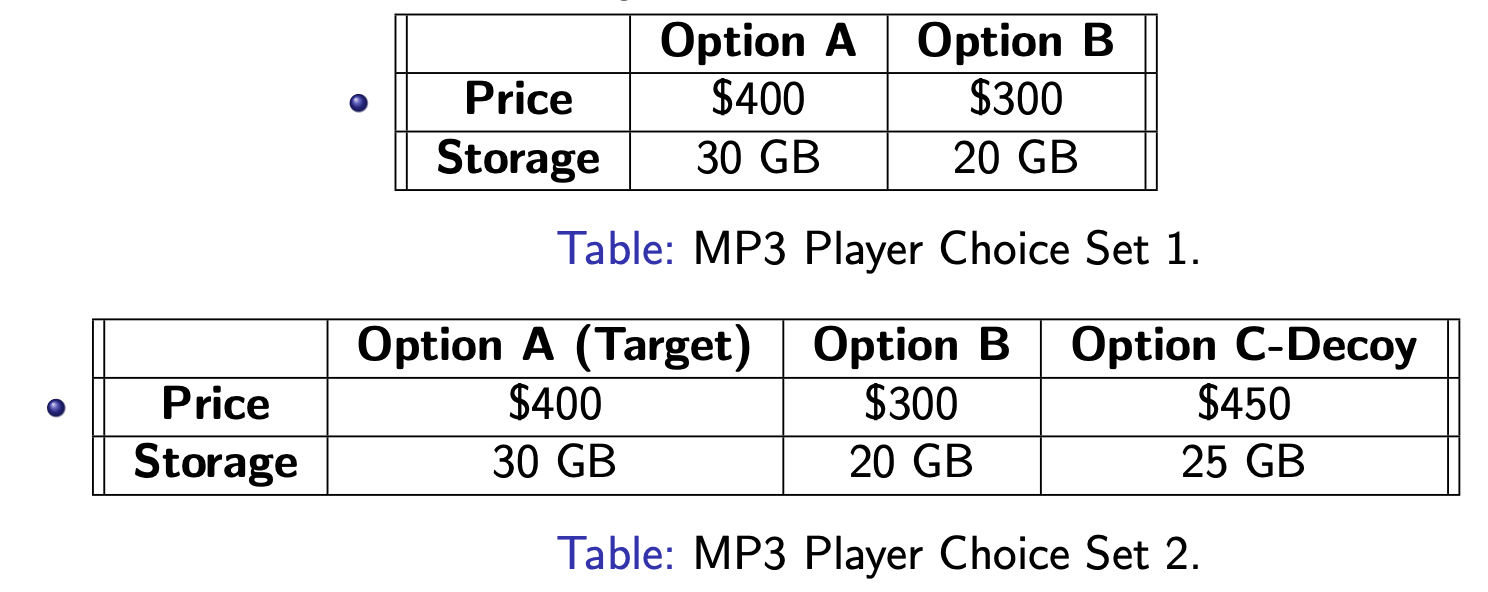
\includegraphics[scale=0.3]{CMNL1.png}
        \caption{Attraction Effect-Decoy Effect}
        \label{}
    \end{figure}\end{center}
    \item \textbf{The compromise Effect:} Middle option gets more share. In particular, in presence of this effect, when adding an extreme option (very high-level or basic product), the share of the middle-level options will increase.
    
    For example, a car-shopper who is given three options:
    \begin{enumerate}[1.]
        \item the low-priced basic model with no extras,
        \item a high-priced fully loaded model with all the extras,
        \item and a mid-priced model with some extras,
    \end{enumerate}
    will most likely choose the middle option.
    \item \textbf{The Similarity Effect:} Adding an item will hurt the market share and perceived preference of the options which are similar to it more than the dissimilar options.
\end{enumerate}
\begin{center}\begin{figure}[htbp]
    \centering
    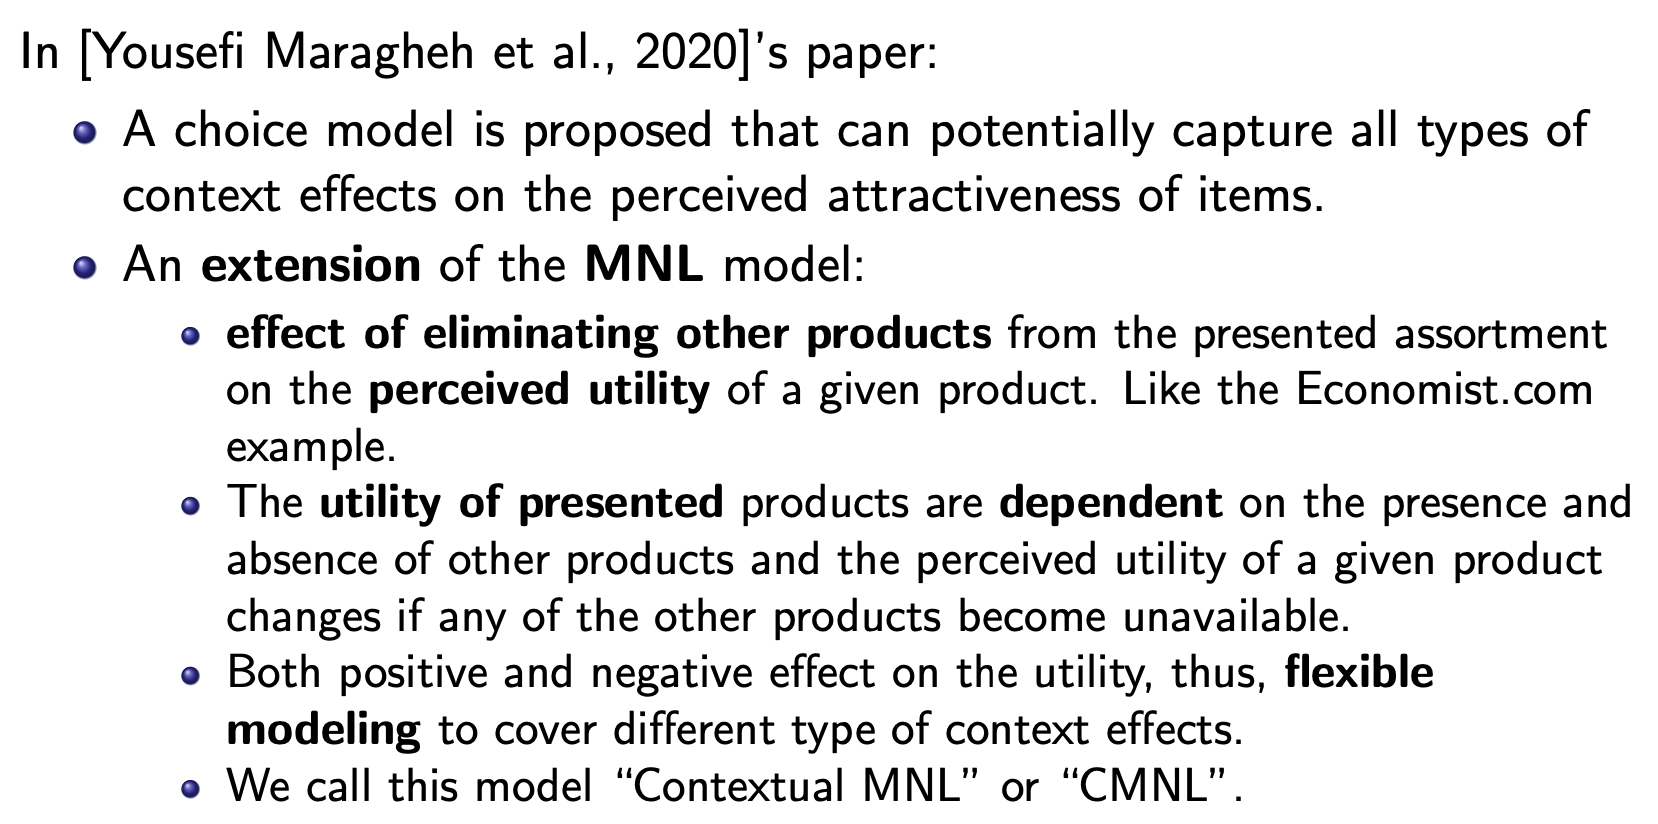
\includegraphics[scale=0.5]{CMNL2.png}
    \caption{CMNL}
    \label{}
\end{figure}\end{center}

\subsection{ Rank List-based Choice Model}
\subsubsection{ Motivation}
\begin{enumerate}[$\bullet$]
    \item Using historical sales data to predict the revenues or sales from offering a particular assortment of products to consumers.
    \item Fitting the ”right” parametric choice model to data are prone to overfitting and underfitting.
    \item The risk of model misspecification and leading to inaccuracies in decision making.
    \item Parametric models are prone to overfitting and underfitting.
    \begin{enumerate}
        \item Too simple model may make practically unreasonable assumptions.
        \item Too complex model can lead to worse performance.
    \end{enumerate}
    \item Need to make a data-driven, nonparametric choice model.
\end{enumerate}

\subsubsection{ Notations}
\begin{center}\begin{figure}[htbp]
    \centering
    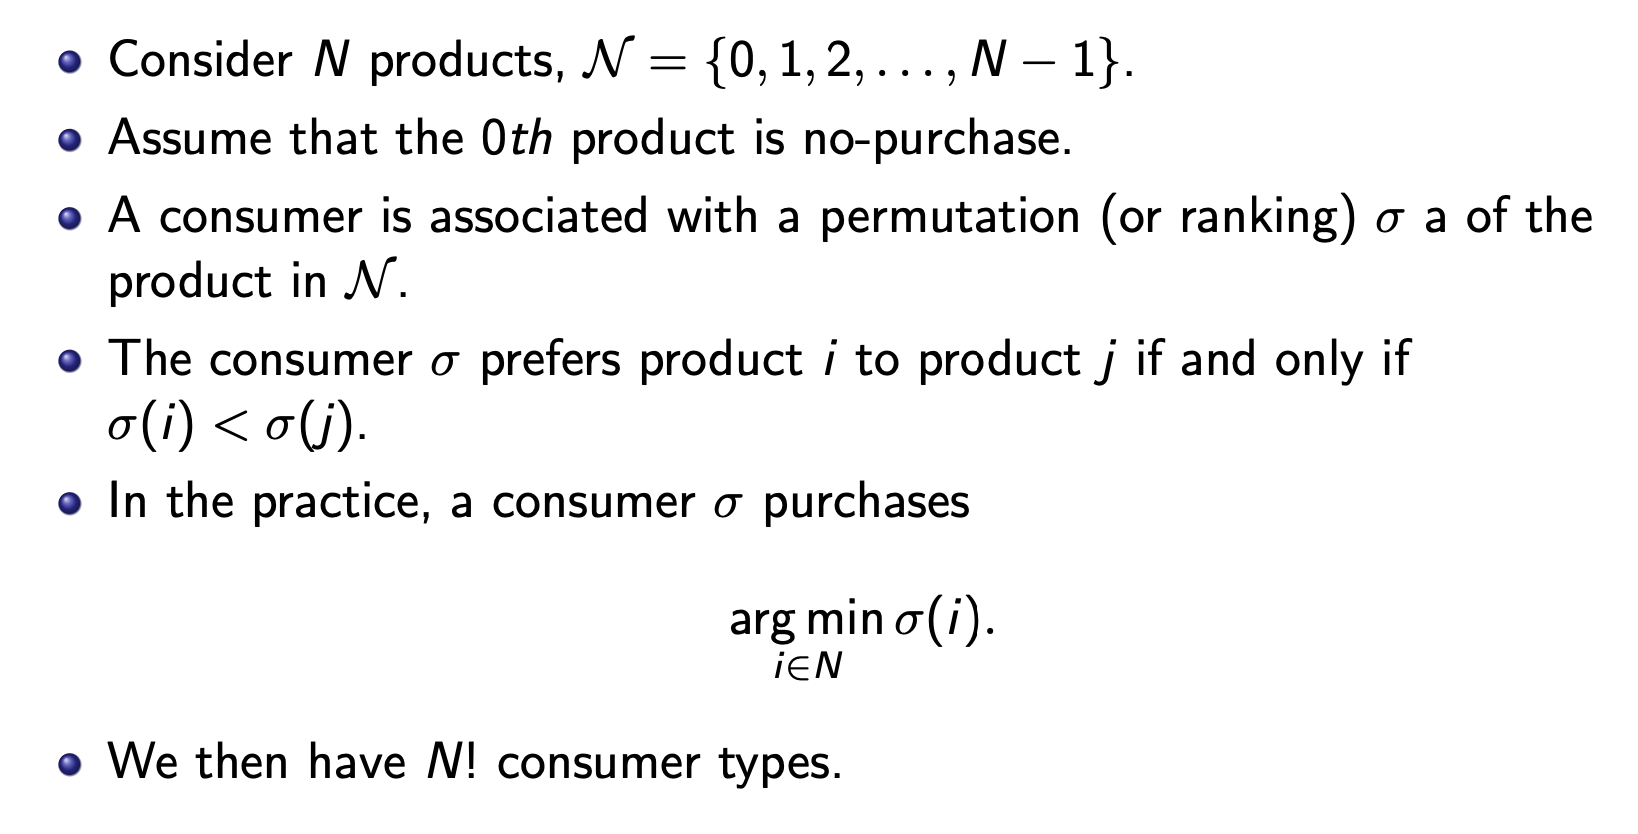
\includegraphics[scale=0.5]{RLCM1.png}
    \caption{Notations}
    \label{}
\end{figure}\end{center}

\subsubsection{ Model}
\begin{center}\begin{figure}[htbp]
    \centering
    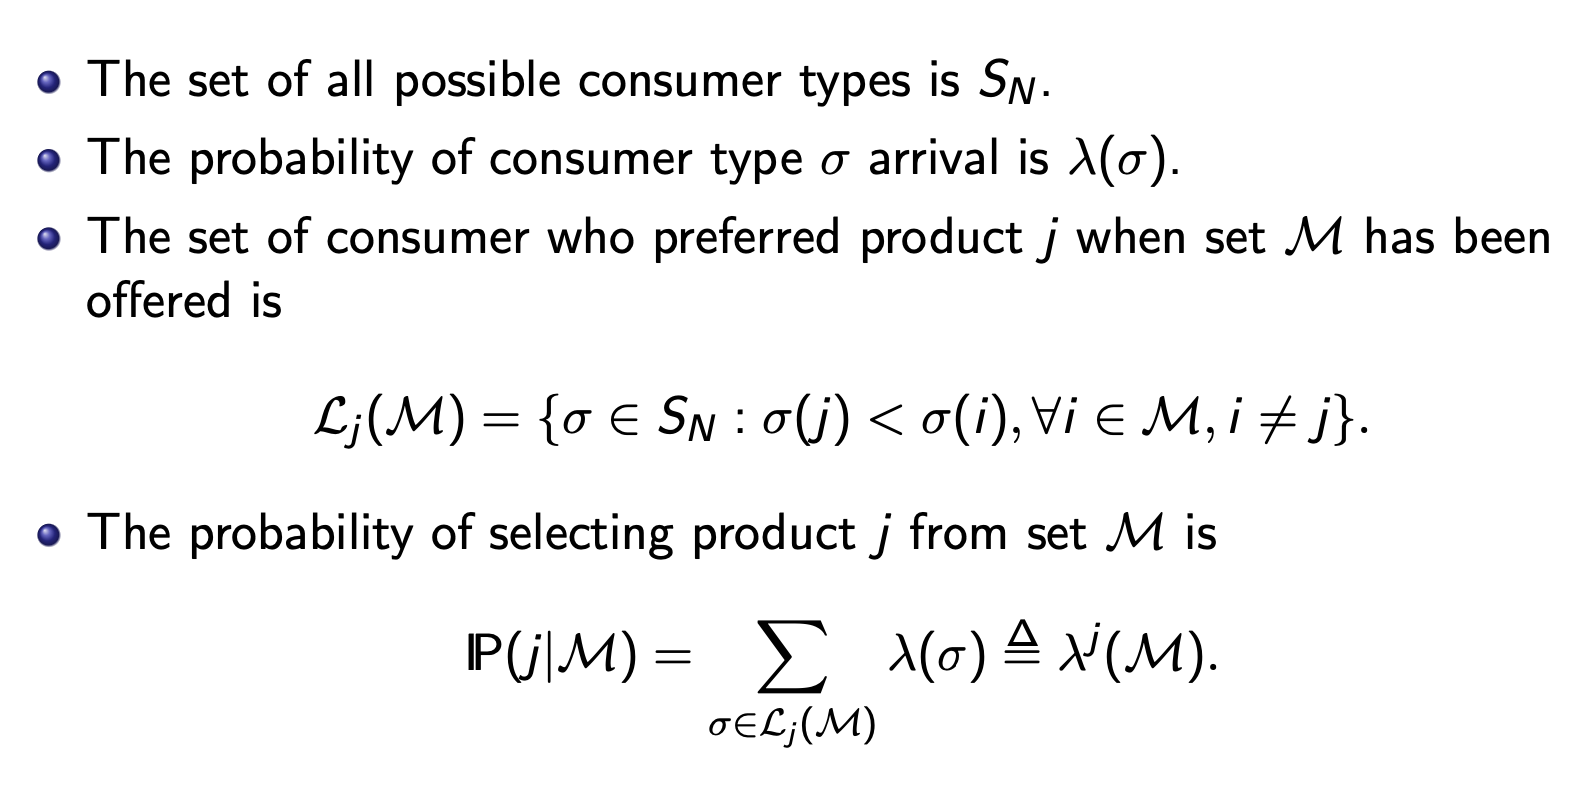
\includegraphics[scale=0.5]{RLCM2.png}
    \caption{Model}
    \label{}
\end{figure}\end{center}
\begin{center}\begin{figure}[htbp]
    \centering
    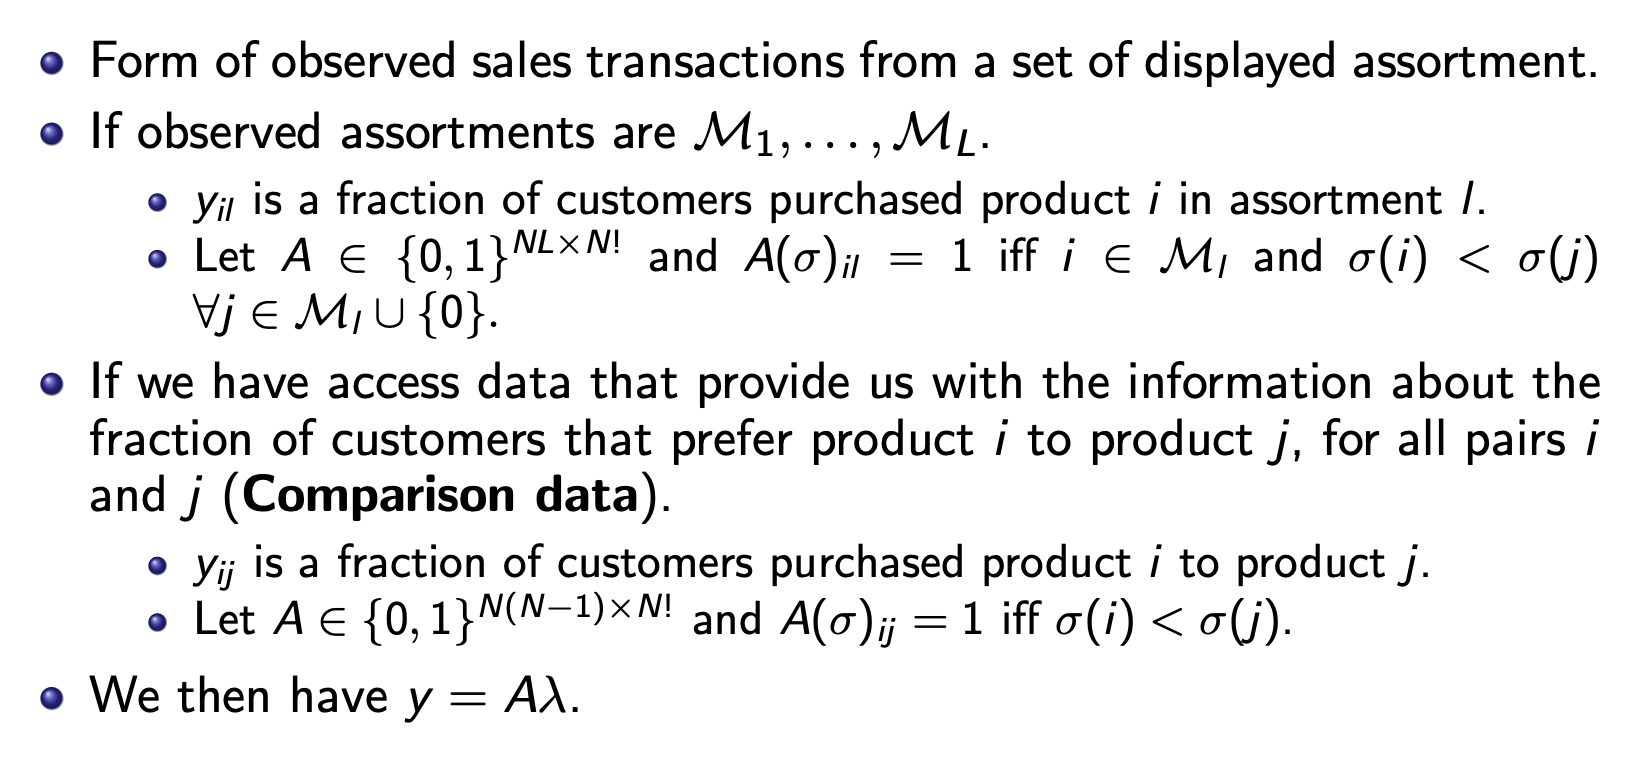
\includegraphics[scale=0.5]{RLCM3.png}
    \caption{Data}
    \label{}
\end{figure}\end{center}
\begin{center}\begin{figure}[htbp]
    \centering
    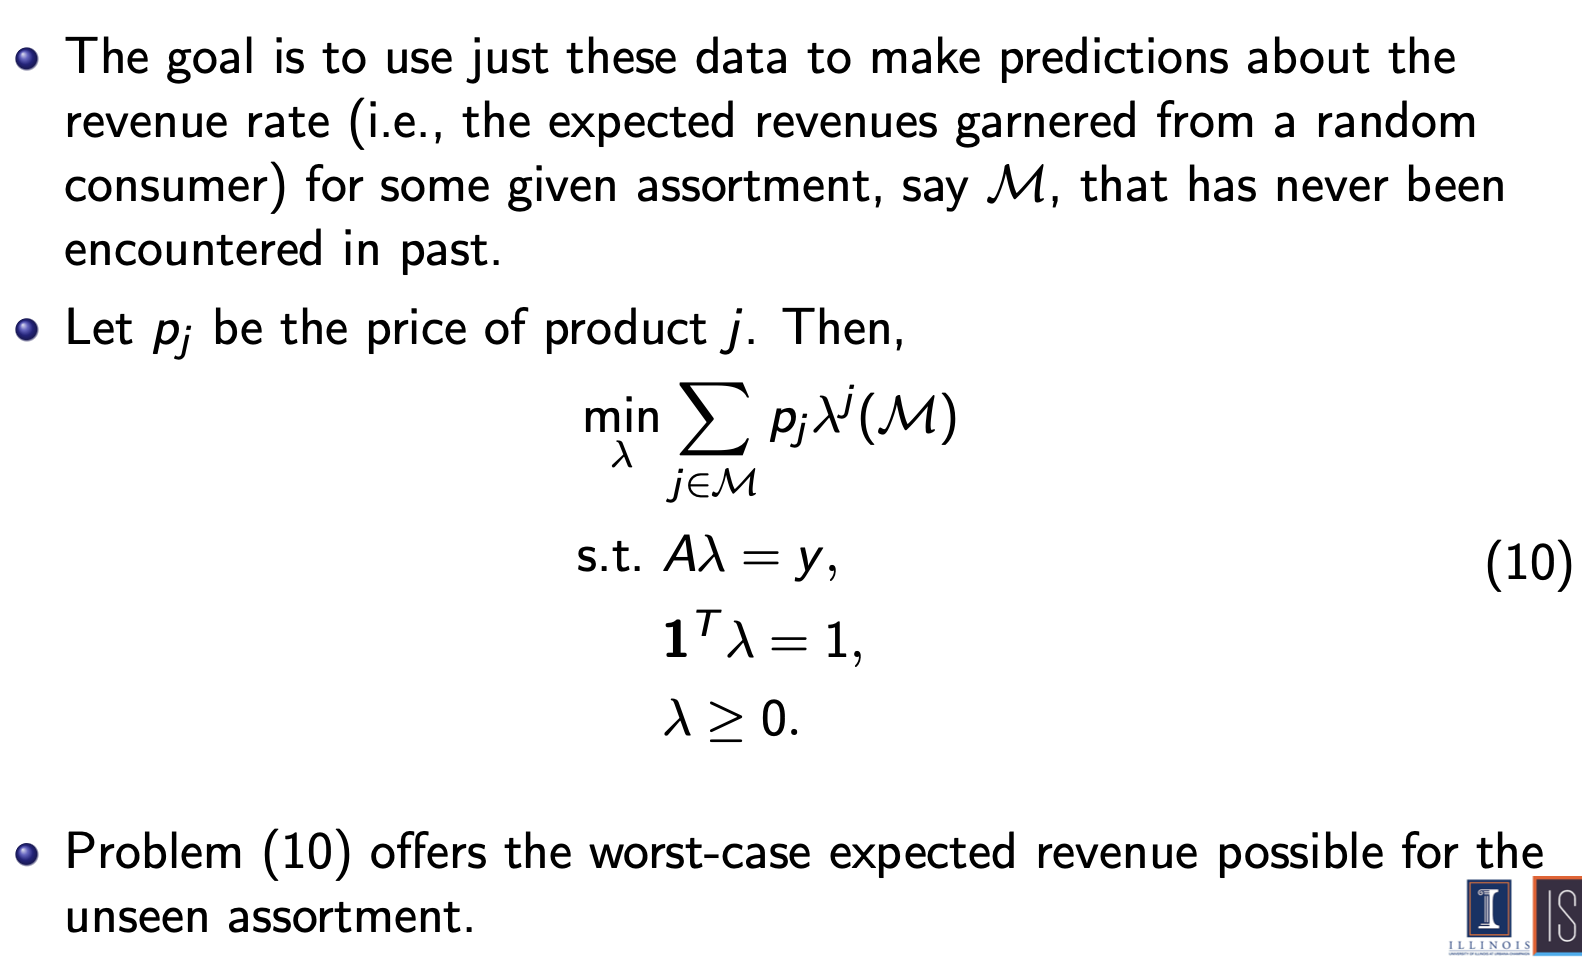
\includegraphics[scale=0.5]{RLCM4.png}
    \caption{Robust Approach}
    \label{}
\end{figure}\end{center}

\subsubsection{ Testing the Performance of Robust Approach}
\begin{center}\begin{figure}[htbp]
    \centering
    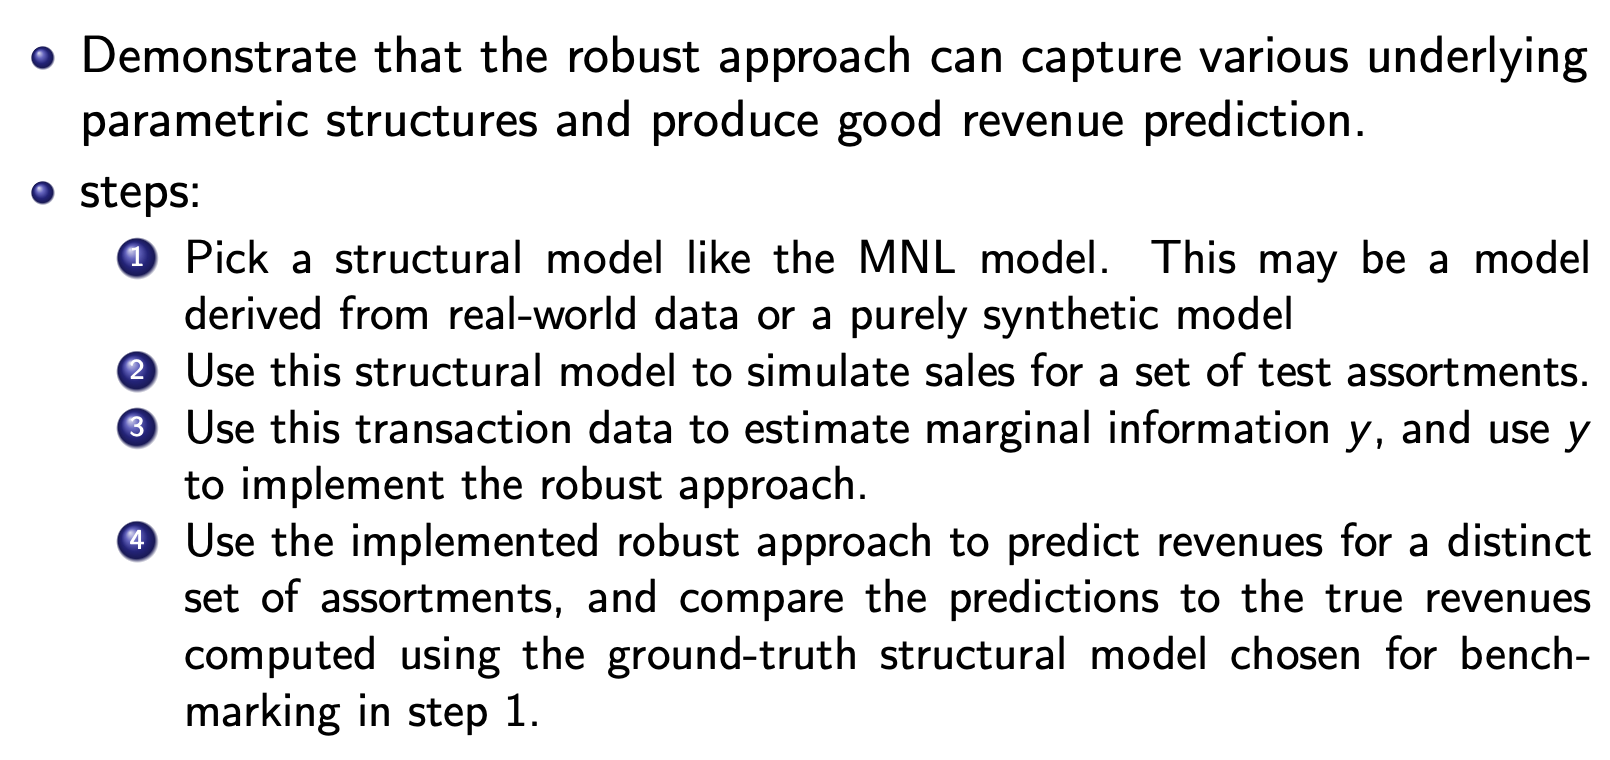
\includegraphics[scale=0.5]{RLCM5.png}
    \caption{Testing the Performance of Robust Approach}
    \label{}
\end{figure}\end{center}
\begin{center}\begin{figure}[htbp]
    \centering
    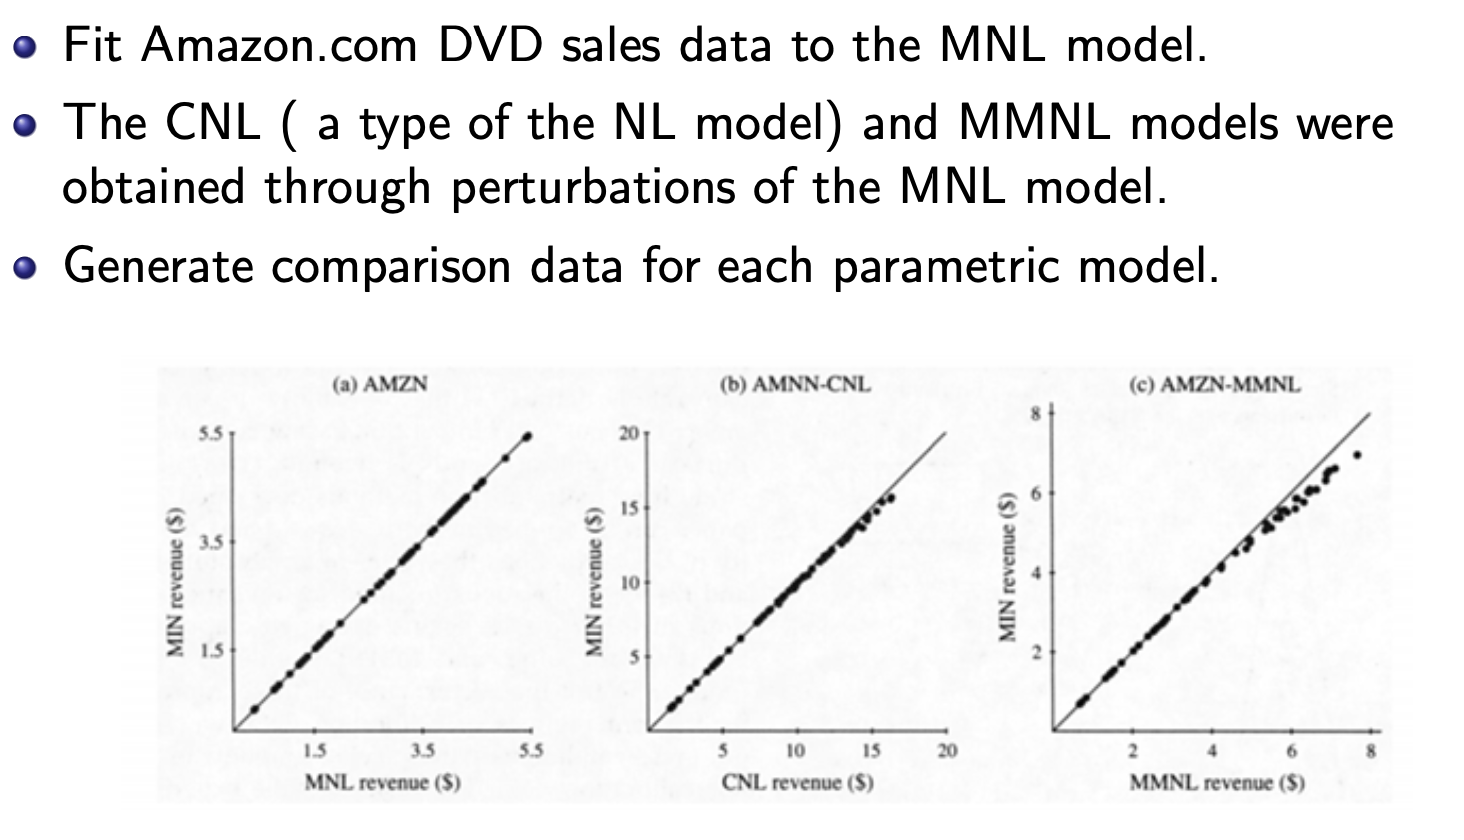
\includegraphics[scale=0.5]{RLCM6.png}
    \caption{Computational Study}
    \label{}
\end{figure}\end{center}

\subsubsection{ Limitations}
\begin{center}\begin{figure}[htbp]
    \centering
    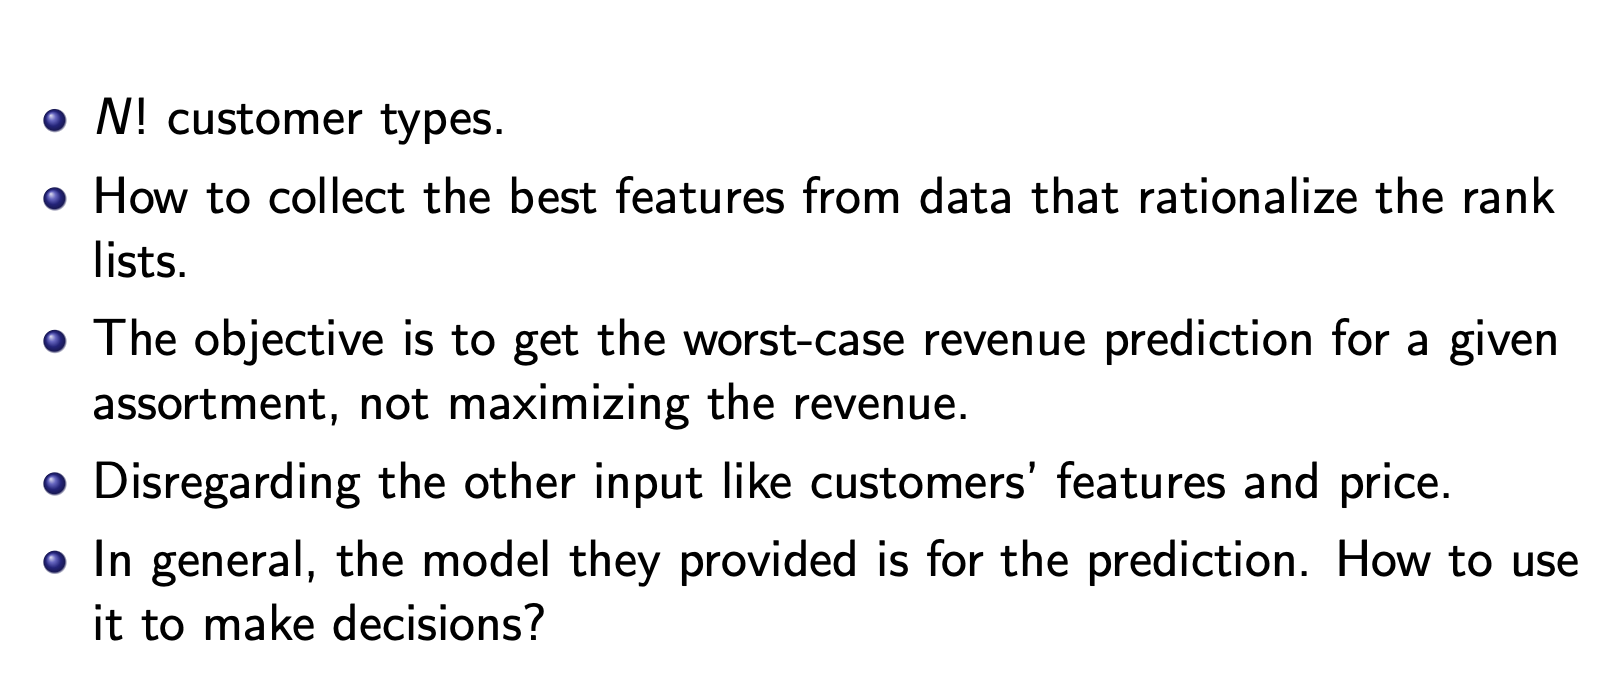
\includegraphics[scale=0.5]{RLCM7.png}
    \caption{Limitations}
    \label{}
\end{figure}\end{center}

\subsection{ Threshold Utility Model}
buy multiple products

\section{ (Joint Pricing and) Assortment Optimization}
\subsection{ Assortment Optimization Problem}
\begin{center}\begin{figure}[htbp]
    \centering
    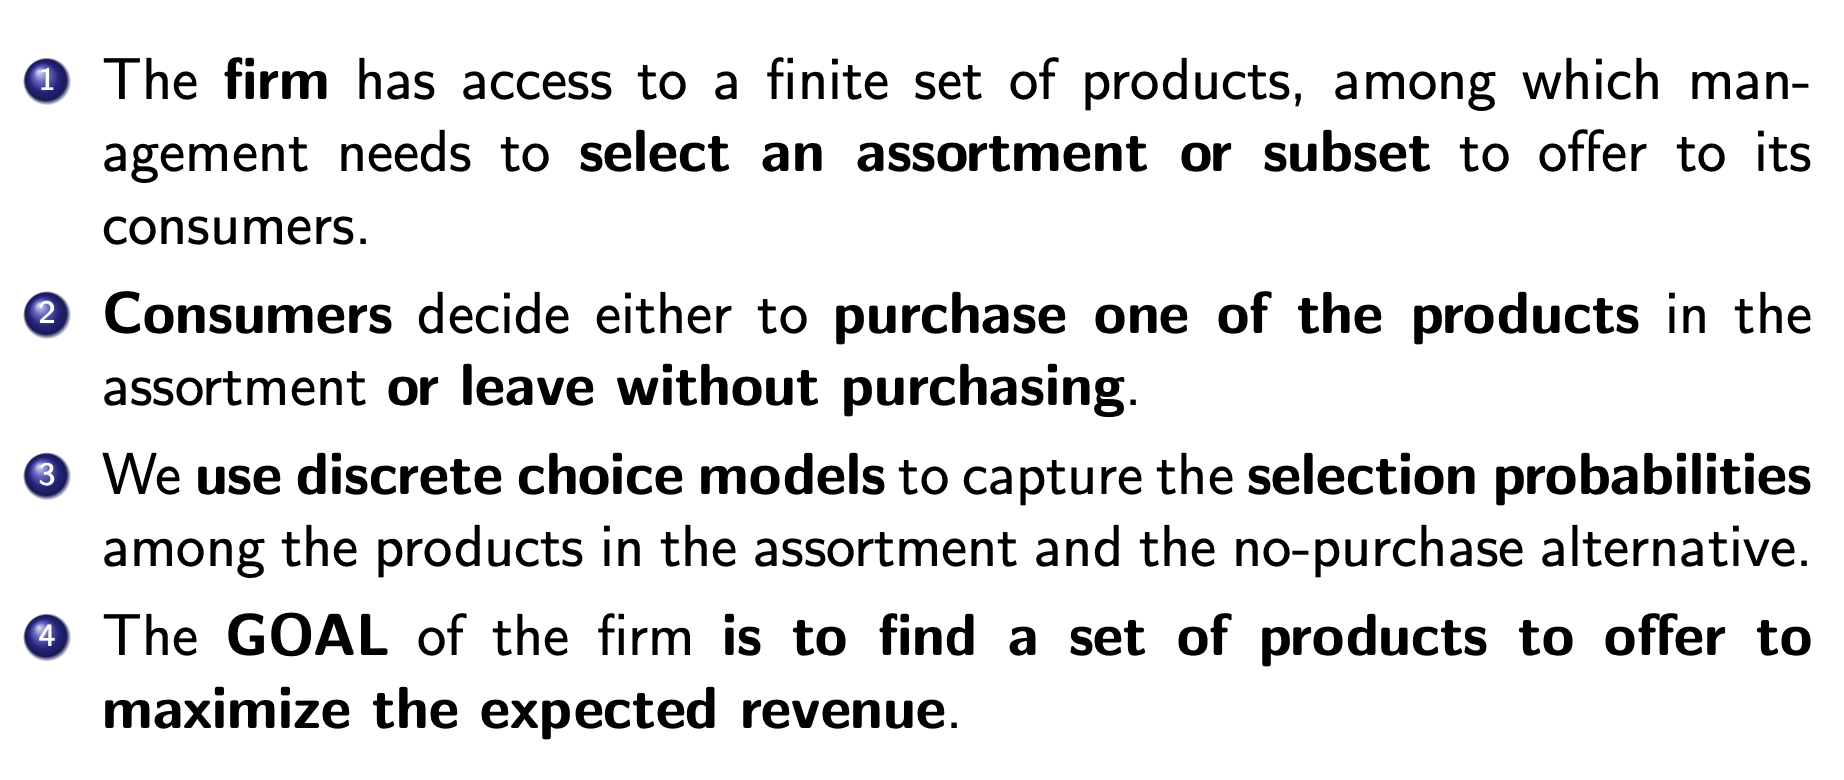
\includegraphics[scale=0.4]{A1.png}
    \caption{What is Assortment?}
    \label{}
\end{figure}\end{center}
The fundamental Trade off in the \underline{Assortment optimization problem (AOP)}:
\begin{enumerate}[$\bullet$]
    \item Broad assortments: demand cannibalization and spoilage,
    \item Narrow assortments: disappointed consumers that may walk away without purchasing.
\end{enumerate}
\subsubsection{ Notations}
\begin{center}\begin{figure}[htbp]
    \centering
    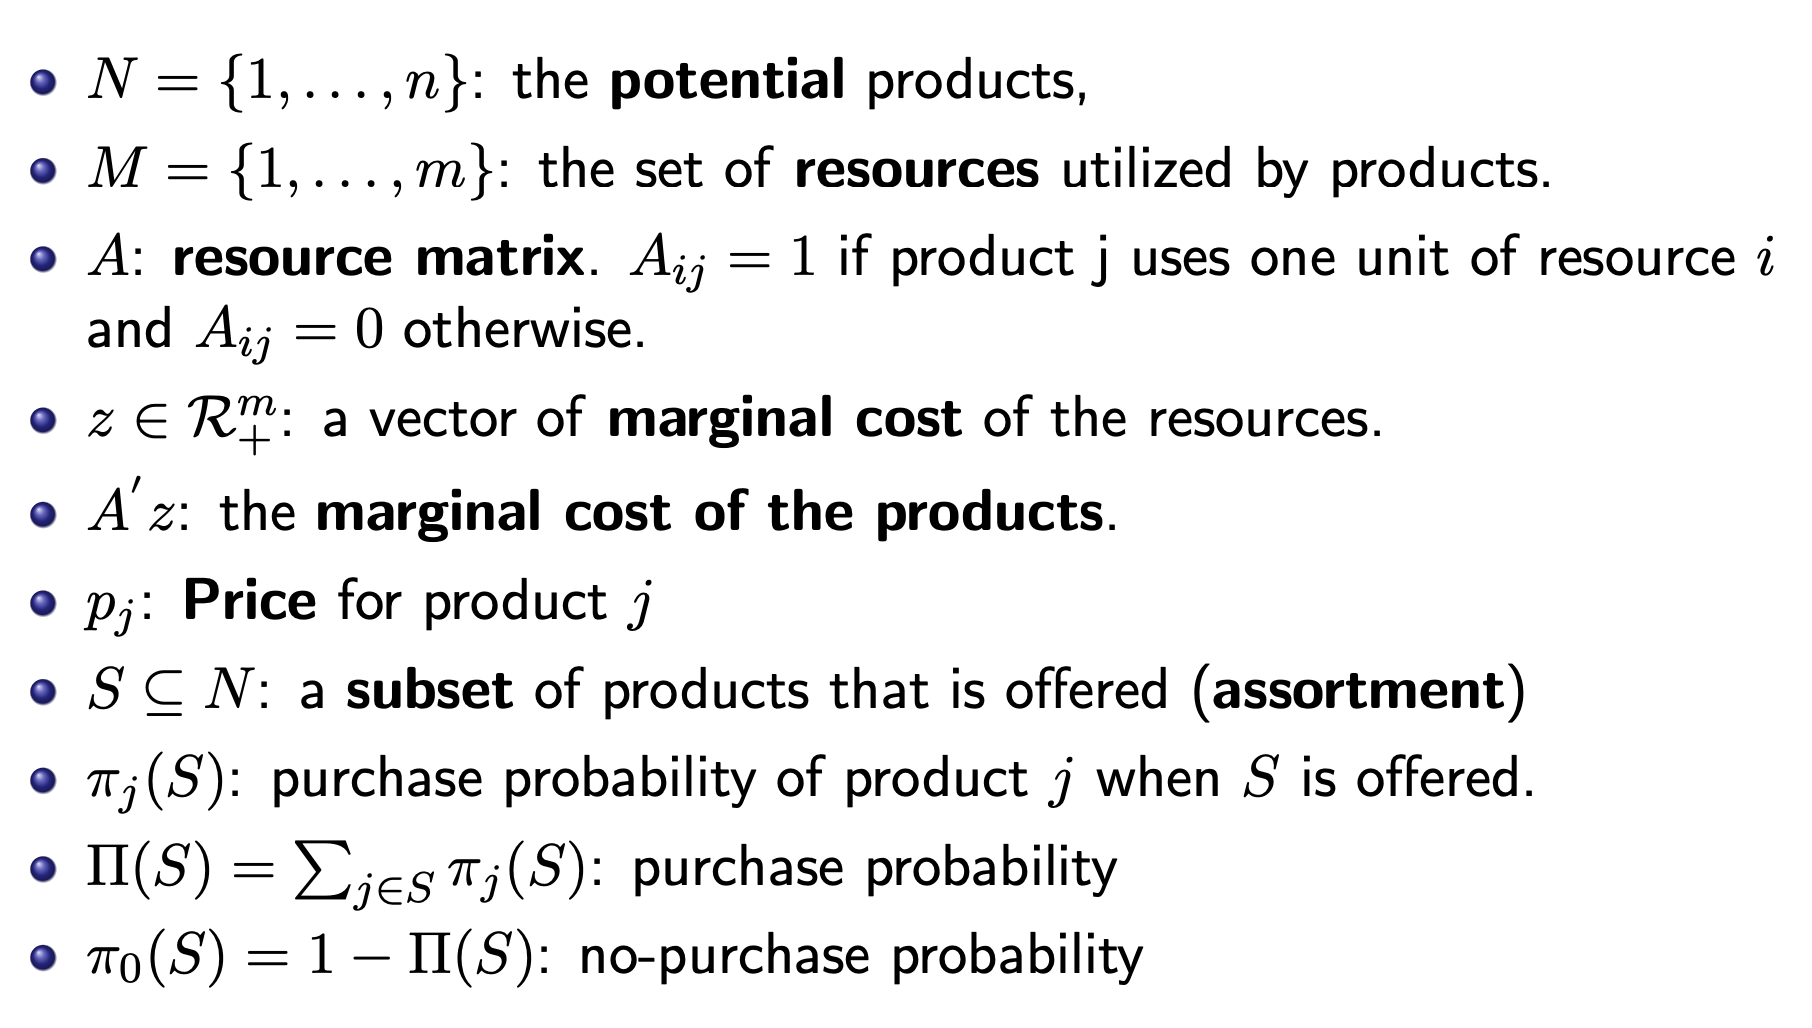
\includegraphics[scale=0.4]{A2.png}
    \caption{Notations}
    \label{}
\end{figure}\end{center}
If we offer $S$, the expected profit from offering subset $S$ is given by:
$$
R\left(S, A^{\prime} z\right):=\sum_{j \in S}\left(p_{j}-A_{j}^{\prime} z\right) \pi_{j}(S)
$$
AOP is finding the $S$ which maximizes $R\left(S, A^{\prime} z\right)$ :
$$
\mathcal{R}\left(A^{\prime} z\right):=\max _{S \subseteq N} R\left(S, A^{\prime} z\right)
$$
For brevity of notation, we will make the transformation $p_{j} \leftarrow p_{j}-A_{j}^{\prime} z$ for all $j \in N$. Also:
\begin{enumerate}[$\bullet$]
    \item $R(S)$ as a short-hand for $R(S, 0)$,
    \item $\mathcal{R}^{*}$ as a short-hand for $\mathcal{R}(0)$.
\end{enumerate}

\subsection{ Pricing and Assortment Planning under the MNL model and Variants}
\subsubsection{MNL Model}
Given an assortment $S \subseteq N$, the random utility $U_{i}$ of product $i \in S$ is
$$
U_{i}=\underbrace{u_{i}\left(p_{i}\right)}_{\text {deterministic part }}+\underbrace{\xi_{i}}_{\text {random part }} .
$$
Define the attraction factor of product $i \in S$ as
$$
v_{i}\left(p_{i}\right)=e^{u_{i}\left(p_{i}\right)} .
$$
When $\xi_{1}, \ldots, \xi_{n}$ are i.i.d. random variables with a Gumbel distribution, through the utility maximization, a consumer chooses product $i \in S$ w.p.
$$
q_{i}=\frac{v_{i}\left(p_{i}\right)}{1+\sum_{j \in S} v_{j}\left(p_{i}\right)}, \quad \forall i \in S .
$$
and the no-purchase probability is
$$
q_{0}=\frac{1}{1+\sum_{j \in S} v_{j}\left(p_{i}\right)}
$$

\subsubsection{ Joint Pricing and Assortment Planning under MNL Model}
The profit of a given assortment $S$ and given prices $\mathbf{p}=\left(p_{1}, \ldots, p_{|S|}\right)$ is
$$
R(\mathbf{p}, S)=\sum_{i \in S}\left(p_{i}-c_{i}\right) q_{i}=\frac{\sum_{i \in S}\left(p_{i}-c_{i}\right) v_{i}\left(p_{i}\right)}{1+\sum_{j \in S} v_{j}\left(p_{j}\right)}
$$
(Costs $\mathbf{c}=\left(c_{1}, \ldots, c_{n}\right)$ are given parameters.)

Step 1: For any given assortment $S \subseteq N$, the optimal prices are
$$
\mathbf{p}^{*}(S) \in \underset{\mathbf{p} \geq \mathbf{c}}{\arg \max } R(\mathbf{p}, S) .
$$
Step 2: Decide the optimal assortment $S^{*}$ by $\mathbf{p}^{*}(S)$.

\subsubsection{ The MNL Model with Linear Deterministic Utilities}
Assume $u_{i}\left(p_{i}\right)=a_{i}-b_{i} p_{i}, \forall i \in S$, where the price sensitivity $b_{i}>0$.

For any given assortment $S \subseteq N$, the pricing problem is
$$
\max _{\mathbf{p} \geq \mathbf{c}} R(\mathbf{p}, S)=\sum_{i \in S}\left(p_{i}-c_{i}\right) q_{i}=\frac{\sum_{i \in S}\left(p_{i}-c_{i}\right) v_{i}\left(p_{i}\right)}{1+\sum_{j \in S} v_{j}\left(p_{j}\right)}
$$
[Hanson and Martin, 1996] have shown that this formulation is not concave in prices.

A transformation:
$$
\begin{gathered}
\frac{q_{i}}{1-\sum_{j \in S} q_{j}}=v_{i}\left(p_{i}\right)=e^{a_{i}-b_{i} p_{i}} \\
\Rightarrow p_{i}(\mathbf{q})=\frac{a_{i}}{b_{i}}+\frac{1}{b_{i}}\left[\log \left(1-\sum_{j \in S} q_{j}\right)-\log \left(q_{i}\right)\right]
\end{gathered}
$$
where $\mathbf{q}=\left(q_{1}, \ldots, q_{|S|}\right)$ is the vector of market shares.

The profit function becomes
$$
R(\mathbf{q}, S)=\sum_{i \in S}\left(p_{i}(\mathbf{q})-c_{i}\right) q_{i}
$$
The pricing problem for a given assortment $S$ becomes
$$
\max _{\mathbf{q}} R(\mathbf{q}, S)
$$
Reference: [Li and Huh, 2011]

\begin{theorem}
    For the MNL model with linear deterministic utilities, for any given $S \subseteq N$, the profit function $R(\mathbf{q}, S)$ is \underline{jointly concave} in each element $q_{i}, \forall i \in S$.
\end{theorem}
\begin{proof}
    Check the Hessian matrix of $R(\mathbf{q}, S)$ and use the preservation of concavity.
\end{proof}

\textbf{Remark:} Theorem 1 is also true under the Nested Logit Model with linear deterministic utilities when the nest dissimilarity parameters $\gamma_{k} \leq 1$ and the products in the same nest has a common price sensitivity.

Reference: [Li and Huh, 2011]

Define a cost-adjusted quality for all products in set $N$ as
$$
\hat{v}_{i}:=\exp \left(a_{i}-b_{i} c_{i}-1\right), \quad \forall i \in N .
$$
When assuming $b_{1}=\cdots=b_{|S|}=b$, the optimal profit of given $S$ is
$$
\rho^{*}(S)=W\left(\sum_{j \in S} \hat{v}_{j}\right) / b
$$
where $W(\cdot)$ is the Lambert W function which is the inverse of $f(x)=x e^{x}=z$, i.e., $W(z)=f^{-1}(z)$.
\begin{lemma}
    $W(z)$ is positive, increasing, strictly concave, and strictly log-concave.
\end{lemma}
When assuming $b_{1}=\cdots=b_{|S|}=b$, the optimal prices of given $S$ are
$$
p_{i}^{*}(S)-c_{i}=\rho^{*}(S)+\frac{1}{b}=\frac{W\left(\sum_{j \in S} \hat{v}_{j}\right)+1}{b},
$$
which is the so-called "equal markup pricing".

The normalized selling quantities (market shares) are
$$
q_{i}^{*}=\frac{\hat{v}_{i} \exp \left(-b \rho^{*}(S)\right)}{1+\sum_{j \in S} \hat{v}_{j} \exp \left(-b \rho^{*}(S)\right)}=\frac{\hat{v}_{i}}{\exp \left(W\left(\sum_{j \in S} \hat{v}_{i}\right)\right)+\sum_{j \in S} \hat{v}_{i}}
$$
References: [Li and Huh, 2011]
















\end{document}







